\chapter{Implementation}

\section{Installing gateways in Furtwangen}

At the beginning of this thesis, \ac{TTNM} already showed one existing \ac{LoRaWAN} gateway in the Furtwangen area.
It was located on top of the \ac{HFU} G building and was installed by a team of students of the Business Informatics (WING) faculty.

However, to make a good geolocation through multilateration for a \ac{LoRaWAN} node, it is necessary to have at least three gateways in range of the node, as shown in \cref{sec:multilateration-basics}.
Thus, the first step was to research and order additional gateways.

Next, the gateways had to be installed in suitable locations.
This was made possible by the many helping hands that were involved in the installation process, as mentioned in \cref{sec:expression-of-thanks}.

\subsection{Researching gateways}

Some gateways that were used in this thesis were ones that were already in the possession of the \ac{HFU}.
Such was the case for the \emph{Dragino LG308 / LG308N} indoor gateways as well as a \emph{RAK7258} indoor gateway.

Additionally, for development purposes, a \emph{Dragino PG1301} gateway was also used.
The PG1301 is designed to be used with a Raspberry Pi and mounts on top of it in typical Raspberry Pi shield fashion.
This allows low-level access to the \ac{LoRa} module on the board, since it can be directly accessed by the Raspberry Pi's serial interface.

Two MikroTik wAP LR8 kit gateways were purchased for the thesis.
They were chosen after recommendation by a member of the \ac{HSN-TTN} team~\cite{hochschwarzwald_smart_net_-_thethingsnetwork_eingesetzte_nodate}.
The MikroTik wAP LR8 kit was a compelling offer due to its low price and the fact that it comes with MikroTik's \emph{RouterOS}, a well-established GUI for configuring networking devices~\cite{mikrotik_mikrotik_nodate}.
However, it came with the caveat that it did not support \ac{LBS}, as was mentioned in \cref{sec:lorawan-lbs}.
A picture of this gateway can be seen in \cref{pic:mikrotik-lr8-kit-gateway}.
The antenna used with the MikroTik wAP LR8 kit is also from MikroTik, which is a 6.5 dBi antenna which can be seen in \cref{pic:mikrotik-antenna-c-building}.

The other gateways that were purchased for the thesis were two \emph{Dragino DLOS8N} outdoor gateways.
This gateway was chosen due to of difficulties in ordering the second MikroTik wAP LR8 kit.
It was readily available at the time of the order and was chosen as a short-term replacement.
It was used even after the second LR8 arrived because the user interface is identical to the one used in the Dragino LG308 gateway which made it easy to set up.
Similar to the LR8, the DLOS8N also has a weatherproof housing for outdoor use.

\subsection{Locations}\label{sec:gateway-locations}

Multiple locations proved themselves to be worth considering when it came to installing new \ac{LoRaWAN} gateways in Furtwangen.
Various factors were considered when choosing these locations, such as availability of a stable (preferably wired) backhaul internet connection as well as the positioning of the gateways.
Only buildings that the \ac{HFU} has liberal access to were considered, since a long-term deployment of the hardware was desirable to avoid makeshift solutions.
Altitude was also a factor that was considered, as a placement at a higher elevation usually allows for a greater range of the gateway, especially in urban areas such as Furtwangen.

\begin{figure}[htbp]
    \centering
    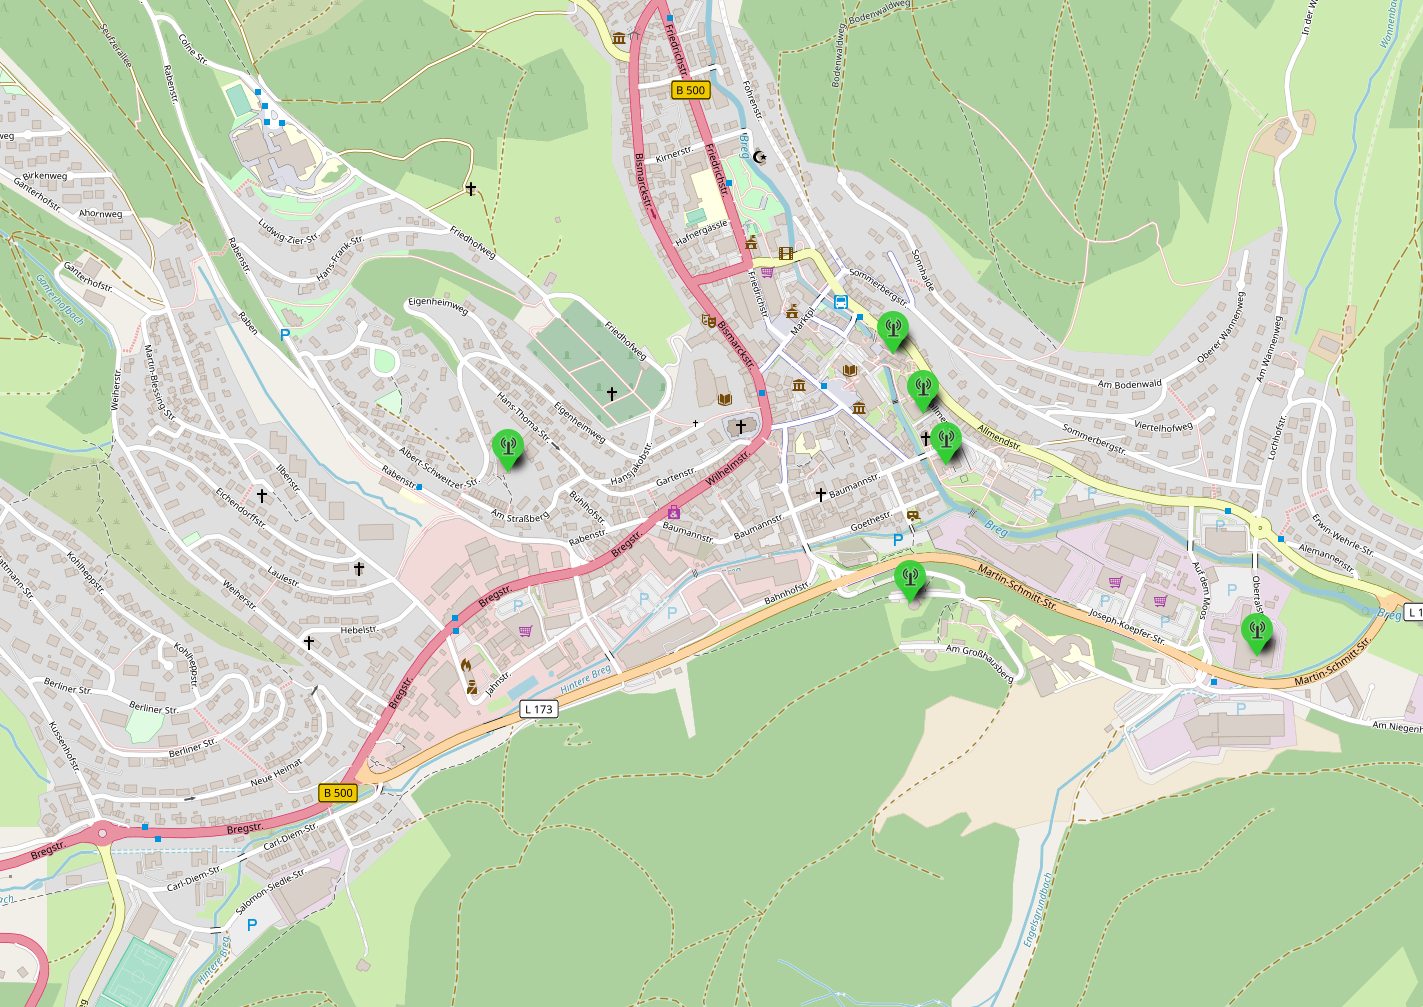
\includegraphics[width=0.8\textwidth]{pictures/hardware/gateway-deployment/gateway_deployment_map.png}
    \caption{
        Overview map of \ac{LoRaWAN} gateways situated in the Furtwangen area.
        This map shows gateways that were placed during this thesis as well as already existing ones~\cite{ttn_mapper_ttn_2023}.
    }\label{pic:gateways-placement-map}
\end{figure}

\Cref{pic:gateways-placement-map} shows the locations of the gateways that were installed during this thesis as well as some that were already present.
The following sections describe and evaluate these final selected sites.

\Cref{sec:gateway-locations-conclusions} will evaluate the chosen locations and give a conclusion on the placement of the gateways.

\subsubsection{\ac{HFU} B and C building}

The first antenna and gateway installed was a Dragino LG308 connected to a MikroTik antenna on top of the \ac{HFU} C building as seen in \cref{pic:mikrotik-antenna-c-building}.
While not as high in altitude as the \ac{GHB} building, it was thought to still be a good location to receive signals from the surrounding area.
The roof of the C building is located in the center of the valley Furtwangen is situated in.
Getting a backhaul connection there proved to be more difficult than anticipated, as the only available connection was a spare fiber optic cable.
However, due to the generosity of the \acl{GHB-NA}, it was possible to use this cable to connect the gateway to the \ac{HFU} network.

A Dragino DLOS8N gateway with an antenna was placed on the roof of the B building because of the existing infrastructure.
This roof was two stories higher than the C building roof, making it a good location for a gateway as well.
The Dragino DLOS8N was used because of its ability to easily be powered by \ac{PoE} and its weatherproof housing.

\subsubsection{\acf{GHB}}

The \ac{GHB} is a popular student dormitory located on the Großhausberg mountainside in Furtwangen~\cite{ghb_netadmins_student_2023}.
Its exposed location and the fact that it is among the highest buildings in the city makes it a good location for putting up a \ac{LoRaWAN} gateway.

The network infrastructure of both the \ac{GHB} and the \ac{ASH} are managed by the \acl{GHB-NA} who are students of \ac{HFU}.
With their help, it was possible to install antennas on the roofs of the \ac{GHB} and \ac{ASH}.

\begin{figure}[htbp]
    \centering
    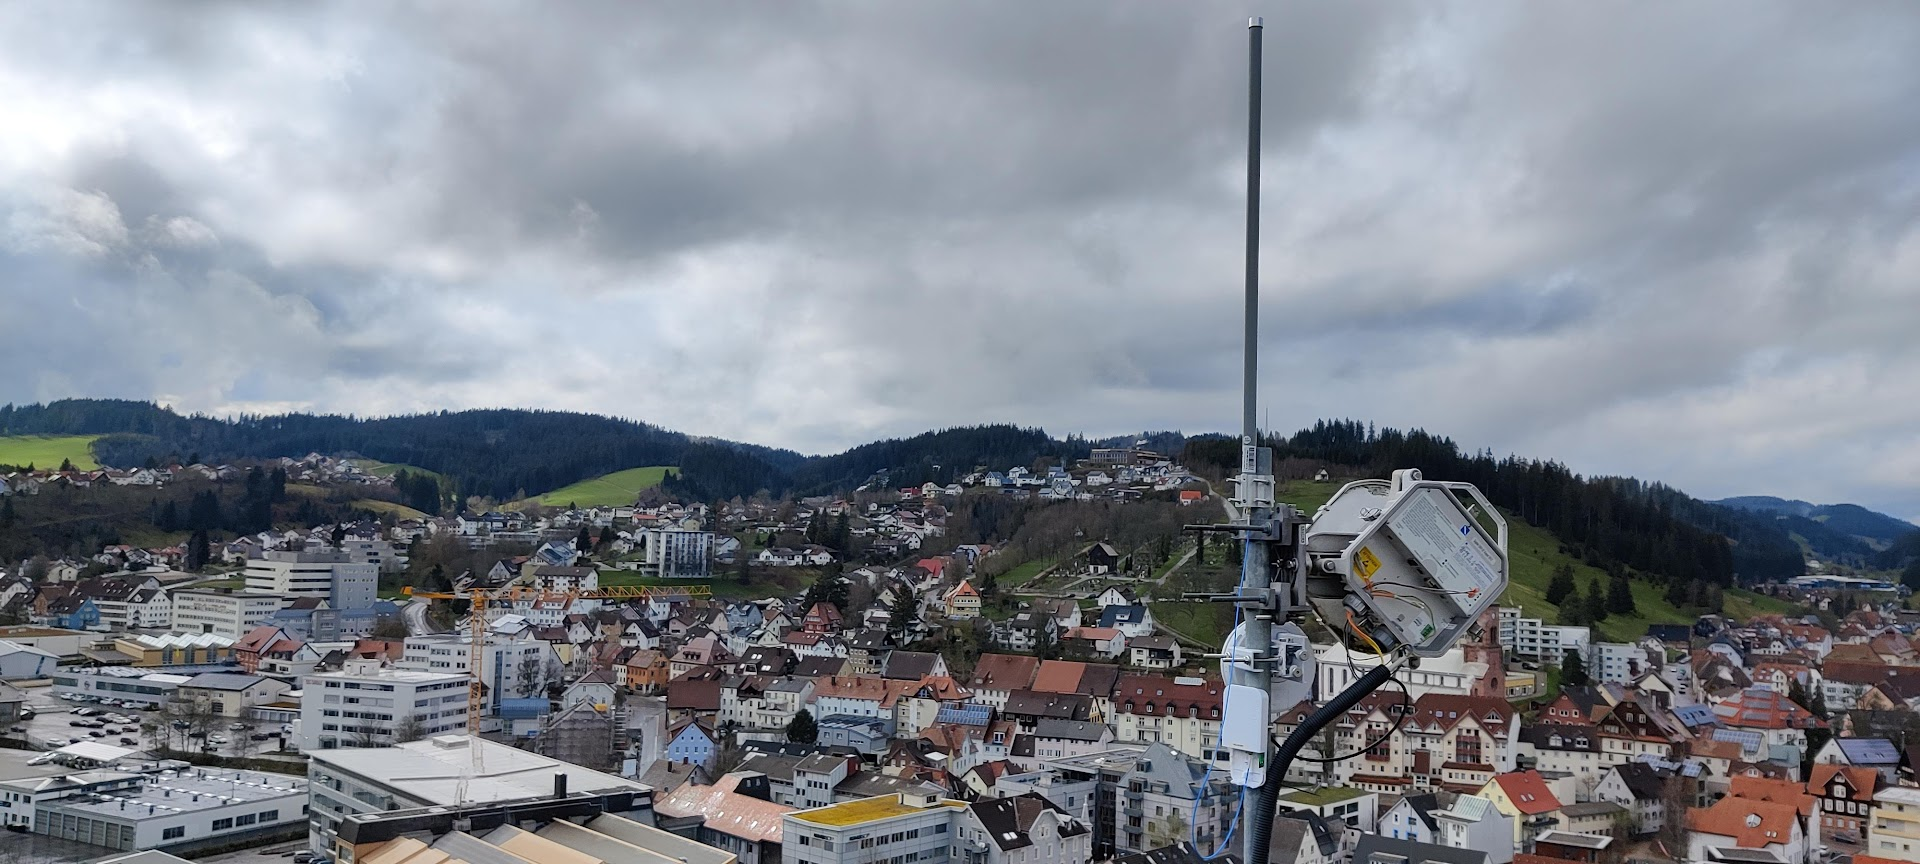
\includegraphics[width=1\textwidth]{pictures/hardware/gateway-deployment/lr8_ghb_installation.jpg}
    \caption{
        The MikroTik LR8 wAP gateway and its antenna installed on the roof of the \ac{GHB}.
        The impressive \ac{LoS} range of the gateway can be seen in the background.
        It can reach most of the valley in which Furtwangen is located.
    }\label{pic:mikrotik-gateway-ghb-installation}
\end{figure}

\Cref{pic:mikrotik-gateway-ghb-installation} shows the installed MikroTik wAP LR8 kit gateway on the roof of the \ac{GHB}.
Again, \ac{PoE} was used to power the gateway since only one cable needed to be put through the existing cable duct.

\subsubsection{\acf{ASH}}

The \ac{ASH} is a former student dormitory located in Furtwangen, which is currently used as housing for refugees.
It sits on a hillside in Furtwangen and was therefore considered a good location for a \ac{LoRaWAN} gateway.
Its network infrastructure is historically managed by the \acl{GHB-NA} and is actually directly connected to the \ac{GHB} building.
This made getting it connected to \ac{HFU} network infrastructure possible even though there were some difficulties with the switches installed in the building as well as crimping the required Ethernet cables.


\begin{figure*}
    \centering
    \begin{subfigure}[t]{0.5\textwidth}
        \centering
        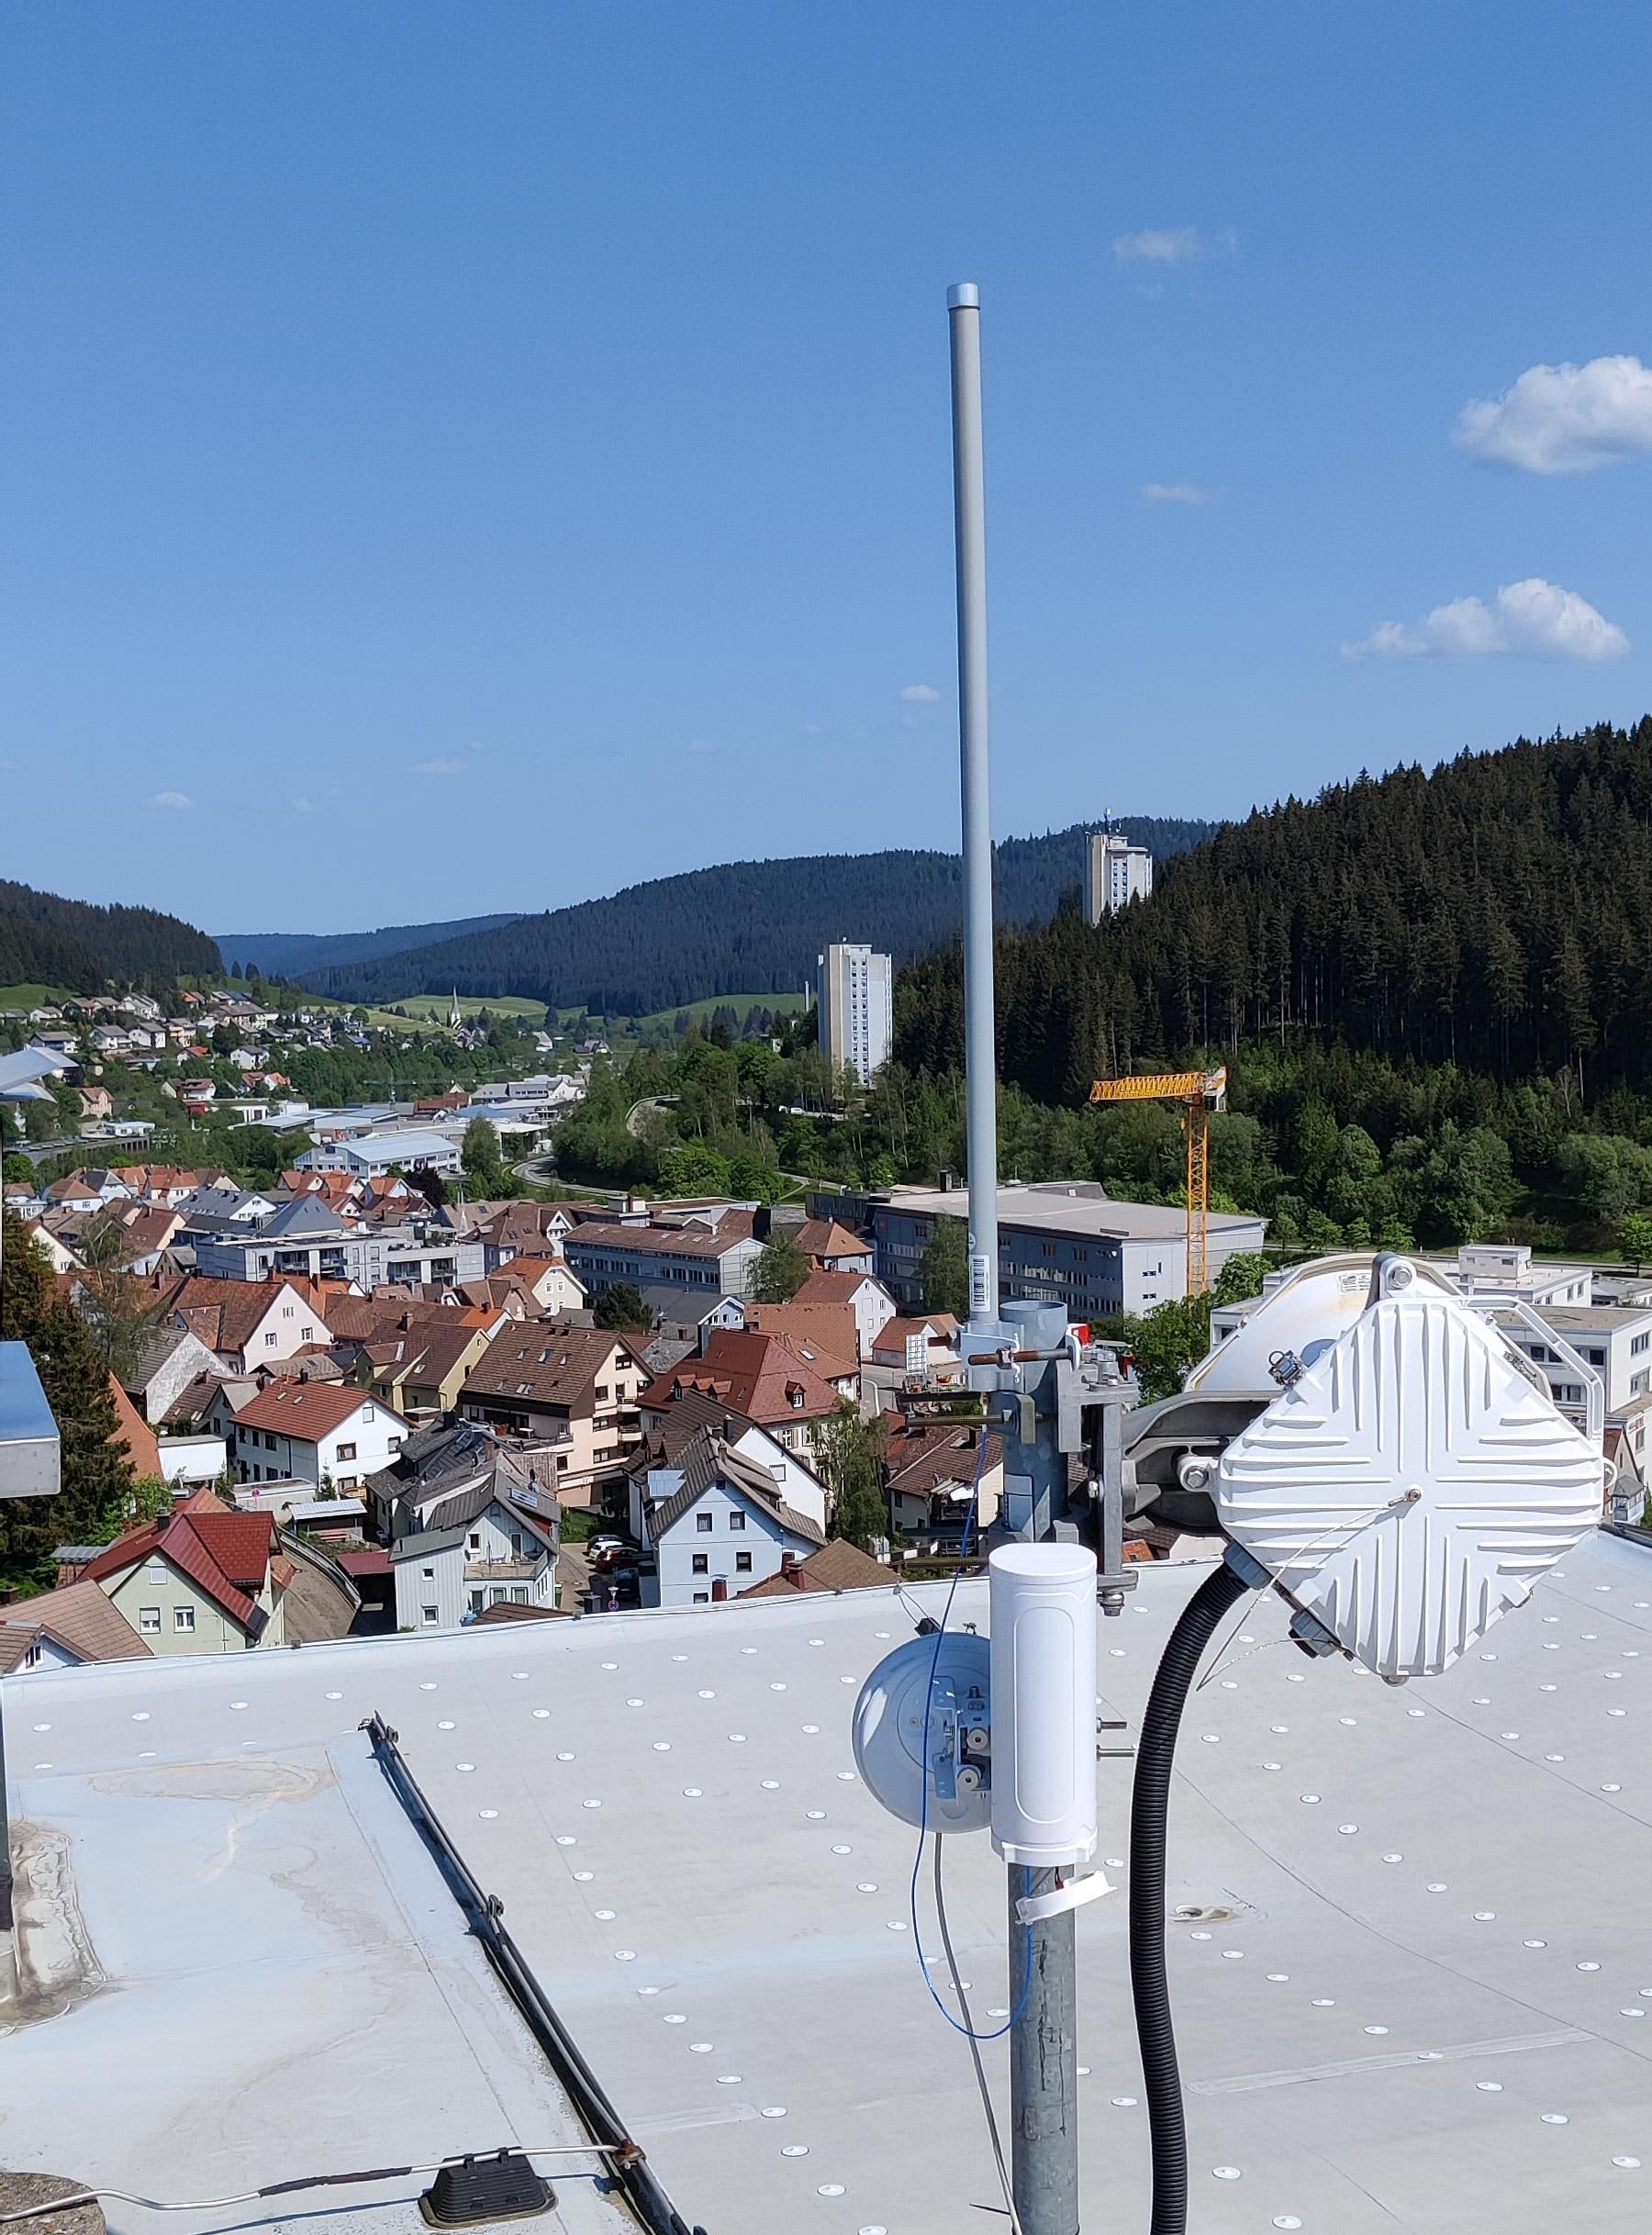
\includegraphics[width=1\textwidth]{pictures/hardware/gateway-deployment/gateway_ash.jpg}
        \caption{
            Installed Dragino DLOS8N gateway with antenna on the roof of the \ac{ASH}.
            Once again, the \ac{LoS} area of the gateway can be seen in the background.
            Also in the background, to the left and right of the gateway's antenna, are the two towers of the \ac{GHB}.
        }\label{pic:dragino-gateway-ash}
    \end{subfigure}%
    ~
    \begin{subfigure}[t]{0.5\textwidth}
        \centering
        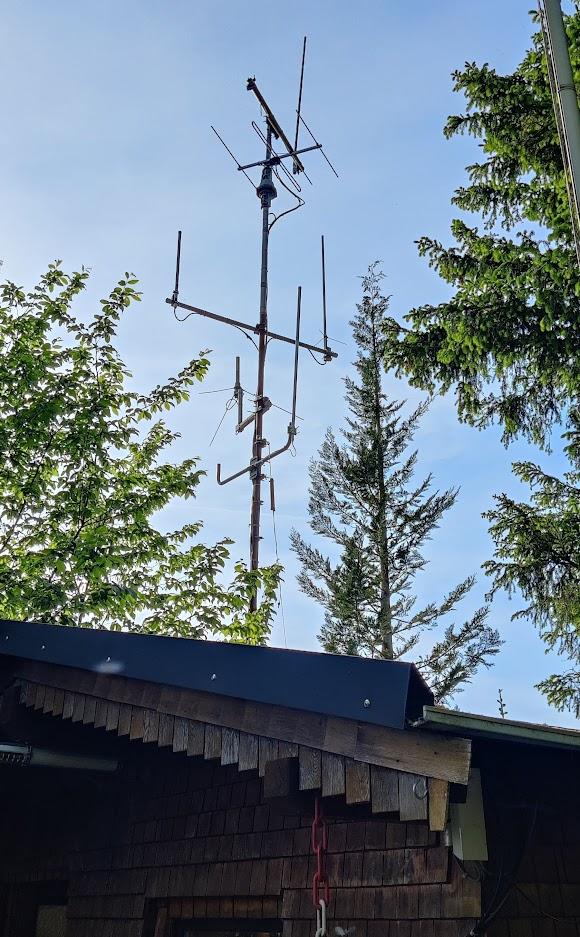
\includegraphics[width=1\textwidth]{pictures/hardware/gateway-deployment/gateway_dl0fis_clubhouse.jpg}
        \caption{
            Antenna installed on the roof of the clubhouse of the \emph{DL0FIS} amateur radio club.
            The antenna has a gain of 8dBi and was connected to a Dragino LG308N gateway.
            It was the most powerful antenna used in this thesis.
            The picture does not show the impressive location of the antenna on a hill between Gütenbach and Furtwangen.
        }\label{pic:antenna-dl0fis-clubhouse}
    \end{subfigure}

    \caption{Pictures of some installed \ac{LoRaWAN} gateways and antennas.}
\end{figure*}

\Cref{pic:dragino-gateway-ash} shows the installed Dragino DLOS8N gateway on the roof of the \ac{ASH}.
This gateway is also powered by \ac{PoE}.
The \acl{GHB-NA} already had a network switch with \ac{PoE} capabilities installed in the \ac{ASH} which made it easy to power the gateway.

\subsubsection{\emph{DL0FIS} amateur radio club station (Neueck, Gütenbach)}

The \emph{DL0FIS} amateur radio club station is located on a hill between Gütenbach and Furtwangen~\cite{dl0fis_clubstation_2023}.
With their friendly support, it was possible to install an antenna on top of their clubhouse as shown in \cref{pic:antenna-dl0fis-clubhouse}.

The exposed location of the clubhouse on a hillside between Gütenbach and Furtwangen was thought to be a good location for a \ac{LoRaWAN} gateway.

\section{Collecting additional \acf{TTNM} data in the Furtwangen area}\label{sec:collecting-additional-ttnm-data}

In order to have more data to work with as far as geolocation calculations are concerned, there was a need to collect more \ac{LoRaWAN}, \ac{RSSI} and \ac{GPS} data that could be synthesized.
This data was especially important for doing geolocation calculations via fingerprinting.

This was done by using \ac{LoRaWAN} devices that were equipped with \ac{GPS} modules and then moving them around Furtwangen.

\subsection{Used \acs{LoRa} devices}\label{subsec:used-lora-devices}

In this section, the \ac{LoRa} devices used for collecting \ac{GPS} data for \ac{TTNM} are described are briefly evaluated.

\begin{figure*}
    \centering

    \begin{subfigure}[t]{0.5\textwidth}
        \centering
        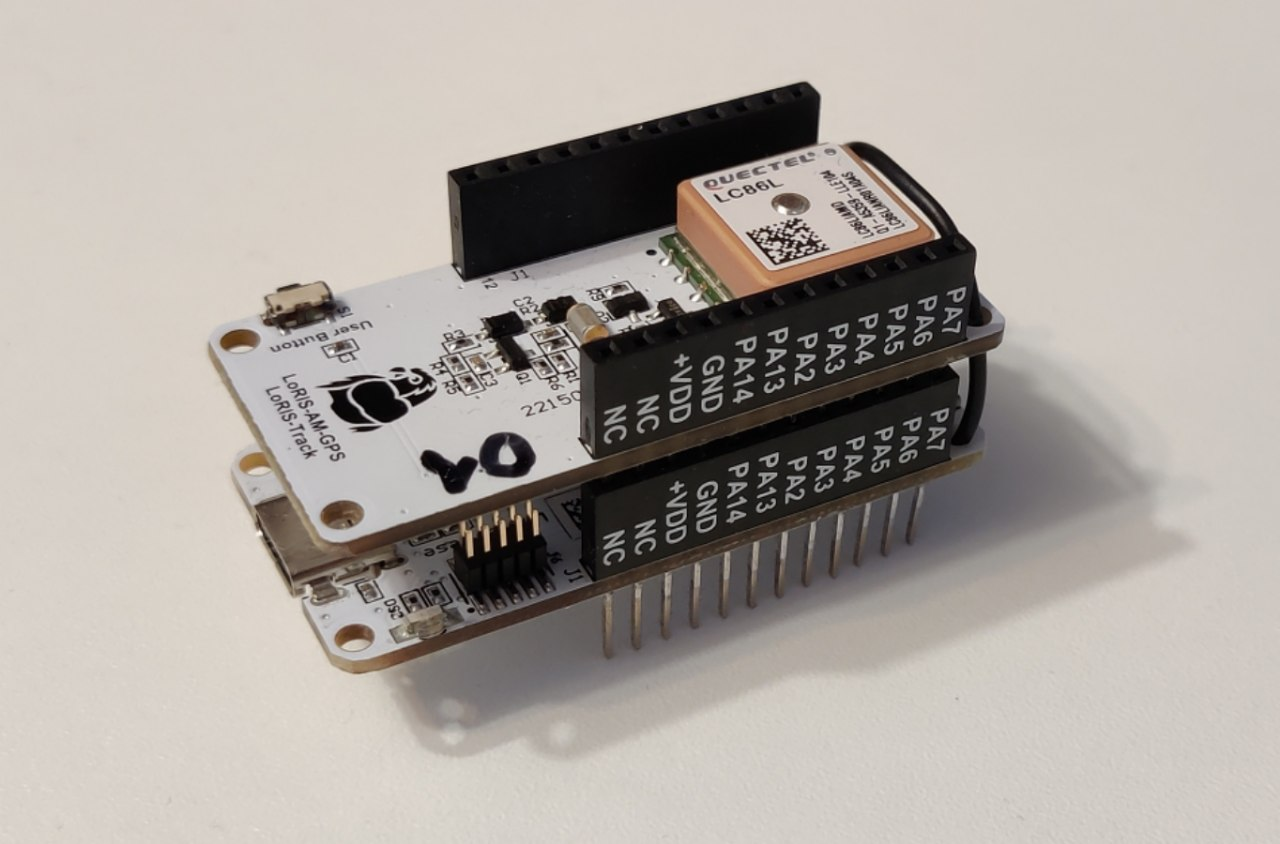
\includegraphics[width=1\textwidth]{pictures/hardware/gps-nodes/loris_bare.jpg}
        \caption{
            ELV-AM-GPS module end device mounted on the LoRIS \ac{LoRaWAN} base.
            The brownish \ac{GPS} module can be seen on the right.
        }\label{pic:loris-node-bare}
    \end{subfigure}%
    ~
    \begin{subfigure}[t]{0.5\textwidth}
        \centering
        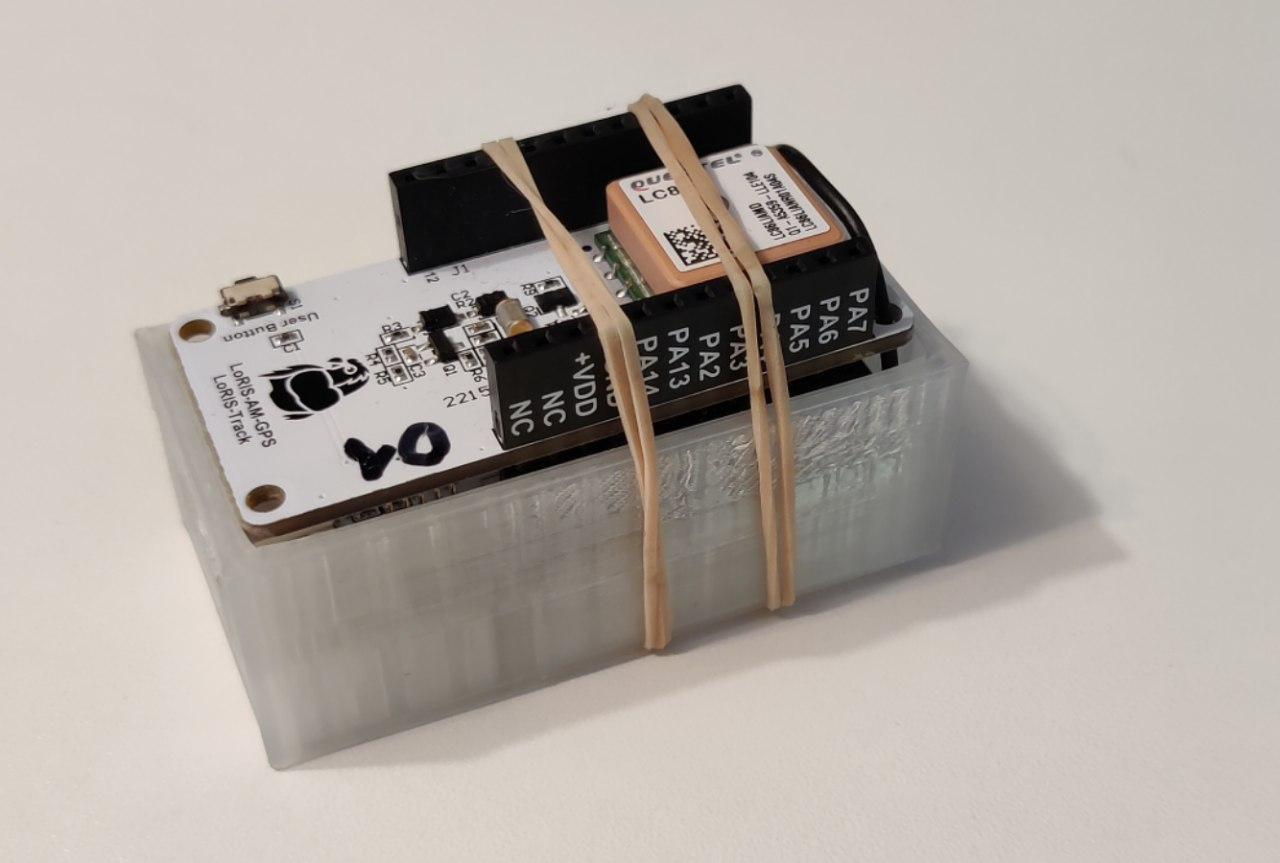
\includegraphics[width=1\textwidth]{pictures/hardware/gps-nodes/loris_with_case.jpg}
        \caption{
            ELV-AM-GPS \ac{LoRaWAN} end device inside a quickly designed 3D printed case.
            The case and the end device are held together by a few rubber bands.
        }\label{pic:loris-node-with-case}
    \end{subfigure}

    \caption{Pictures of the ELV-AM-GPS end device.}
\end{figure*}

\subsubsection{ELV LW experimental platform}\label{subsubsec:elv-lw-experimental-platform}

The ELV LW experimental platform was the \ac{LoRaWAN} node out of the ones used during this thesis that worked best out of the box as far as overall usability is concerned.
The ELV LW experimental platform consists of a base module called ELV-BM-TRX1 and a number of different sensor modules that can be stacked on top of it as seen in~\cref{pic:loris-node-bare}\cite{elv_elektronik_ag_elv-lw-base_2023}.
It has a USB-C port, which made powering the tracker with an external power bank simple.

There are several other modules that can be stacked on top of the base, such as a CO\textsubscript{2} or temperature sensor.
Battery operation is possible by stacking a battery module on top of the base.
Unfortunately, the \ac{GPS} module consumes too much power to be used with the battery module.

Little had to be done in order to begin using the base with the additional \ac{GPS} module ELV-AM-GPS~\cite{elv_elektronik_ag_elv-track_2022}.
Flashing the firmware using a tool provided by the manufacturer was the first step.
Additionally, the \ac{OTAA} credentials provided in the box of the base LoRIS module had to be entered into \ac{TTN}.

To make the board a little more robust, a 3D printed case was designed in Fusion 360 and printed as can be seen in~\cref{pic:loris-node-with-case}.

\subsubsection{ELV \acs{GPS} Tracker}\label{subsubsec:elv-gps-tracker-implementation}

\begin{figure}[htbp]
    \centering
    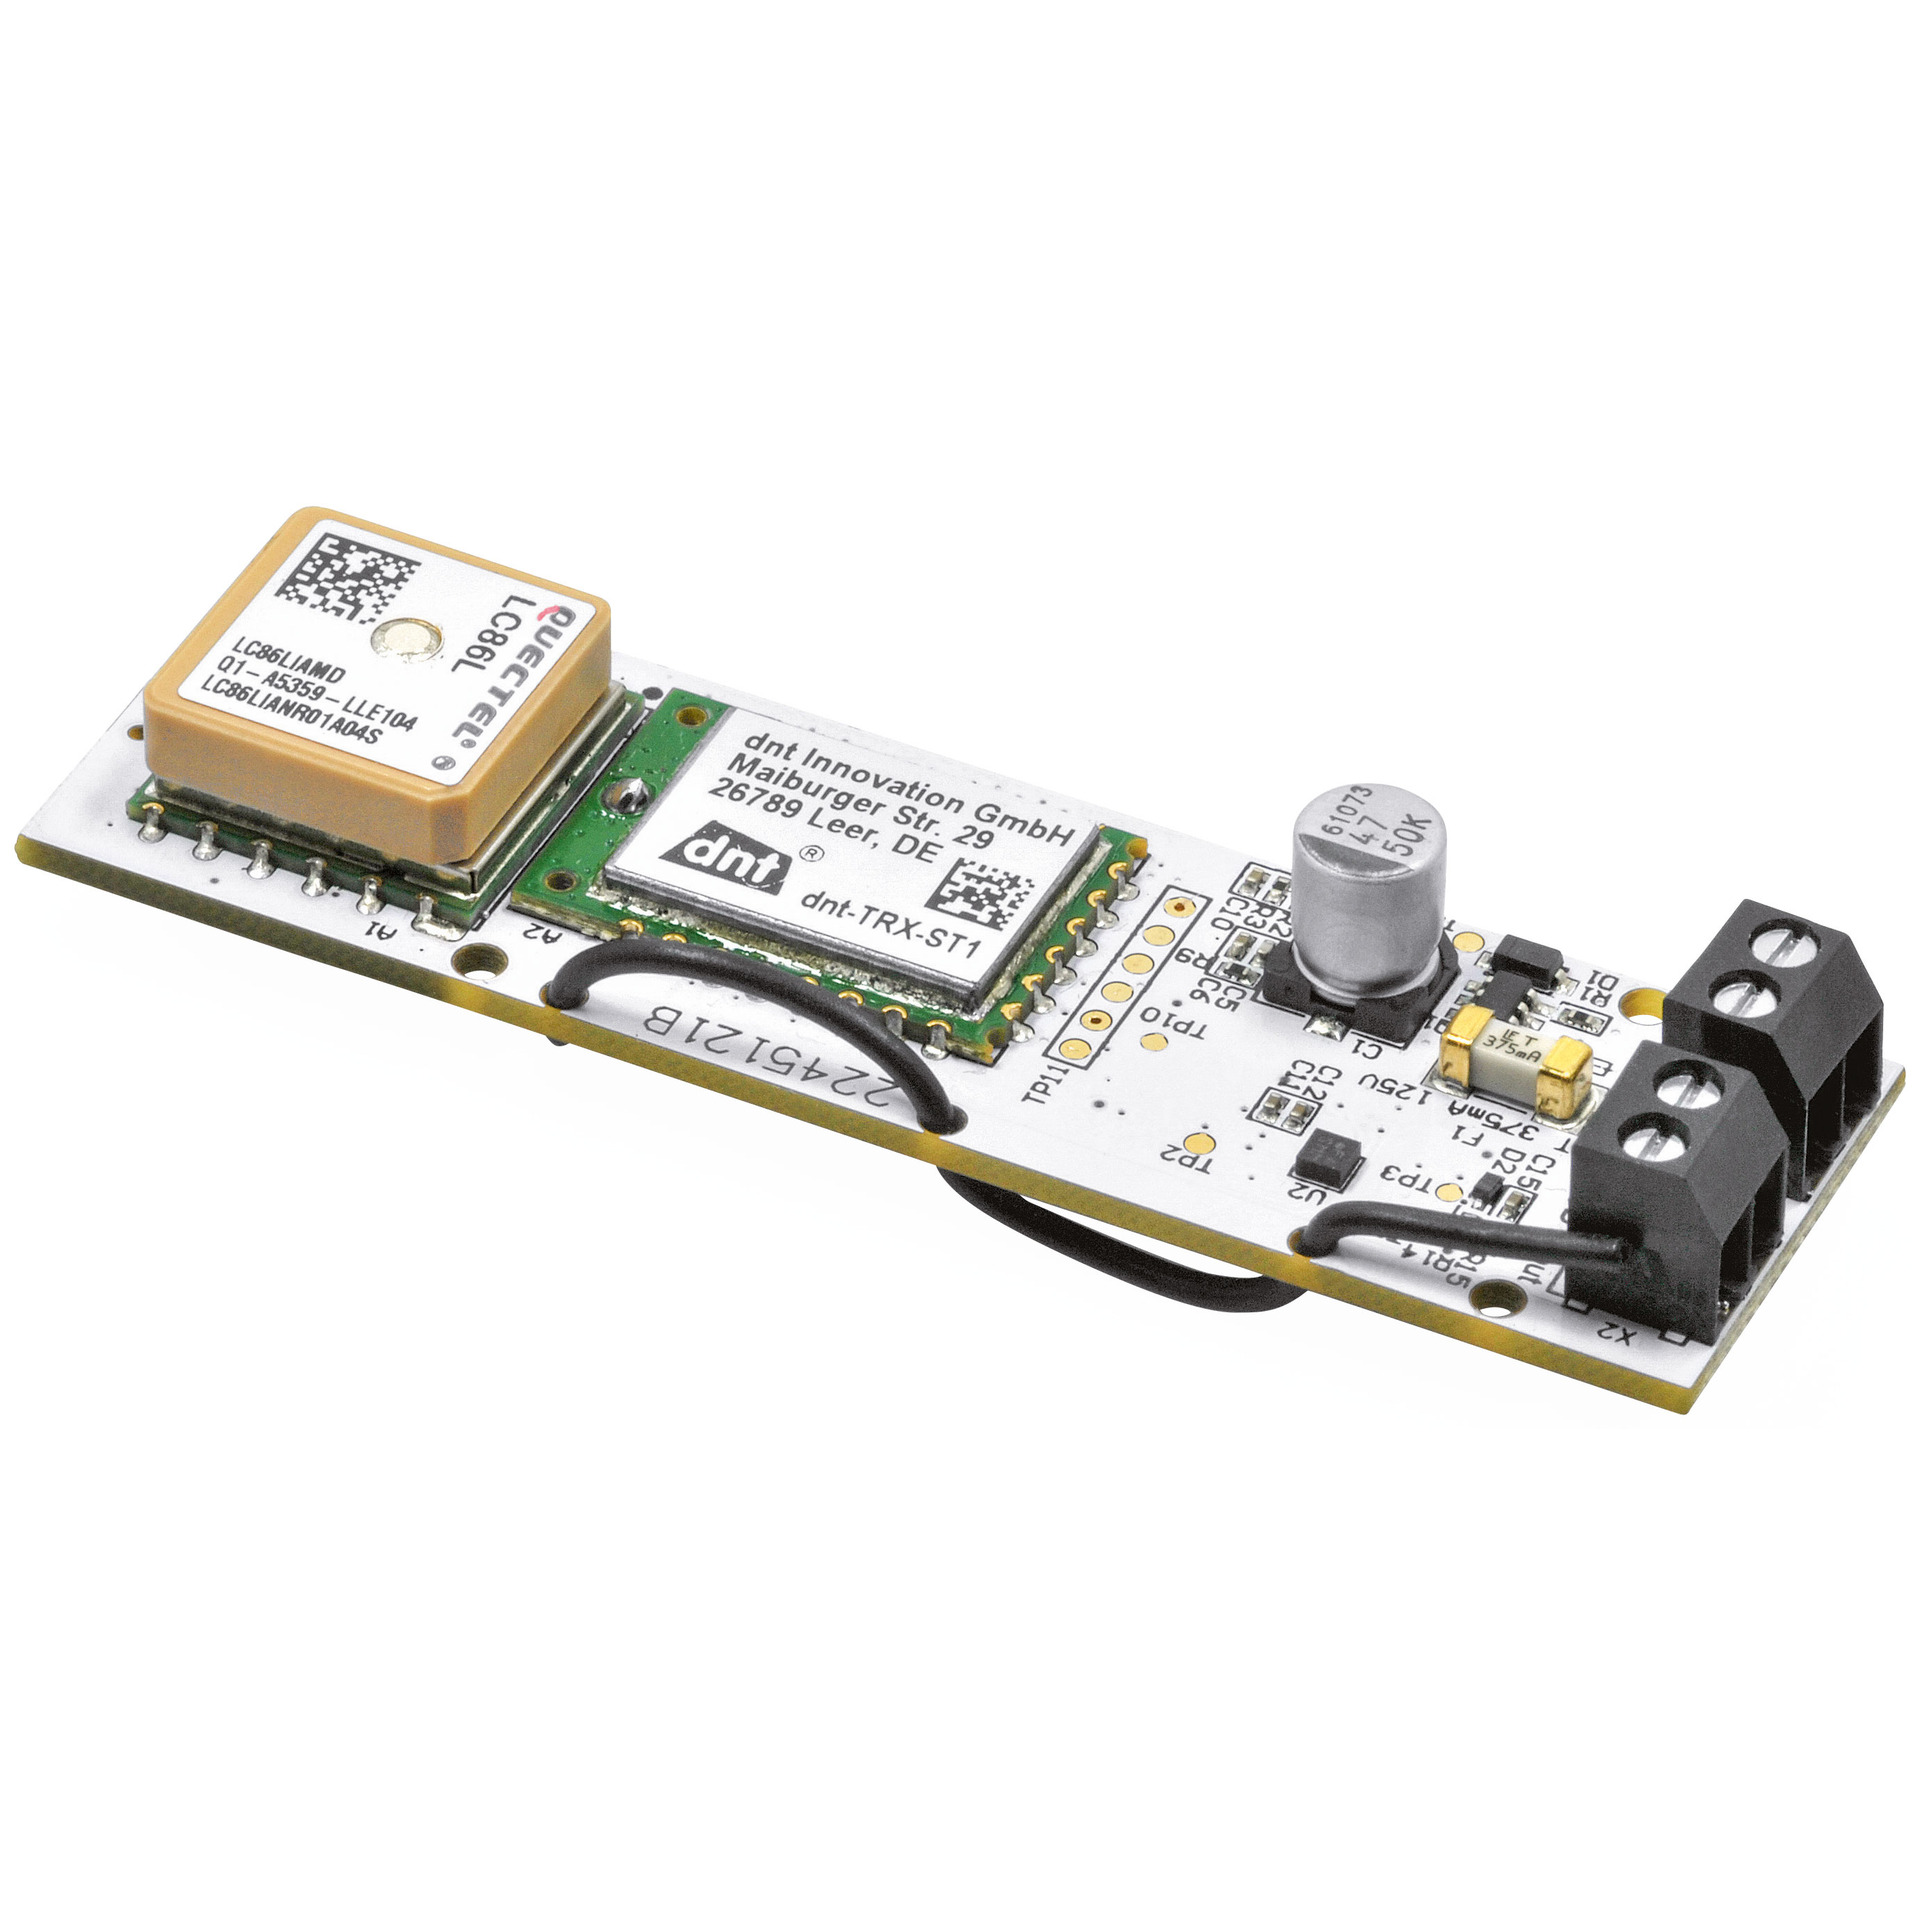
\includegraphics[width=0.4\textwidth]{pictures/hardware/gps-nodes/ELV-LW-GPS1.jpg}
    \caption{
        ELV-LW-GPS1 \ac{LoRaWAN} node~\protect\cite{elv_elektronik_ag_elv_2023}.
        The brownish \ac{GPS} module, similar to the one in \cref{pic:loris-node-bare}, can be seen on the left.
        It uses a similar \ac{LoRa} module as the ELV LW experimental platform.
        The header on the right is used to connect the 5 to 40V power supply as well as an optional physical contact to start a localization on demand.
    }
\end{figure}

The ELV-LW-GPS1 is another \ac{LoRaWAN} node designed to be used as a \ac{GPS} tracker.
Usability-wise, it was similar to the ELV LW experimental platform described in~\cref{subsubsec:elv-lw-experimental-platform}.

It requires a power source that can range from 5 to 40 V, which makes it flexible in terms of power supply.
For example, it can be used with a car battery, which usually has a voltage of 12V.

Finding a power source to be able to use it for this thesis was a challenge.
While it can be powered by a 9V battery, those usually have a low capacity and are not rechargeable.
However, due to the lack of alternatives several such 9V batteries were used for data collection during this thesis.

\Cref{subsec:gnss-power-usage} used this node to compare the power consumption of the \ac{GPS} module to the power consumption of a \ac{LoRa} transmission.

\subsubsection{Heltec HTCC-AB02S}\label{subsubsec:heltec-htcc-ab02s}

The \emph{Heltec HTCC-AB02S} is a \ac{LoRaWAN} node with a small OLED screen and a built-in \ac{GPS} module~\cite{heltec_automation_cubecell_2020}.
The package sounds very nice, but while the \ac{LoRa} module worked flawlessly, the same cannot be said for the \ac{GPS} module.
\Cref{pic:heltec-htcc-ab02s} shows the device.
Programming the device with the \ac{VSC} plugin \emph{PlatformIO} was quite easy.

The \ac{GPS} module was not able to get a reliable fix on its own, even after ordering and using an external GPS antenna.
This seemed to be a hardware problem, since other users could get fixes reliably with external \ac{GPS} antennas.
Because of those problems, the Heltec HTCC-AB02S was not used for data collection during this thesis.

\begin{figure*}
    \centering

    \begin{subfigure}[t]{0.5\textwidth}
        \centering
        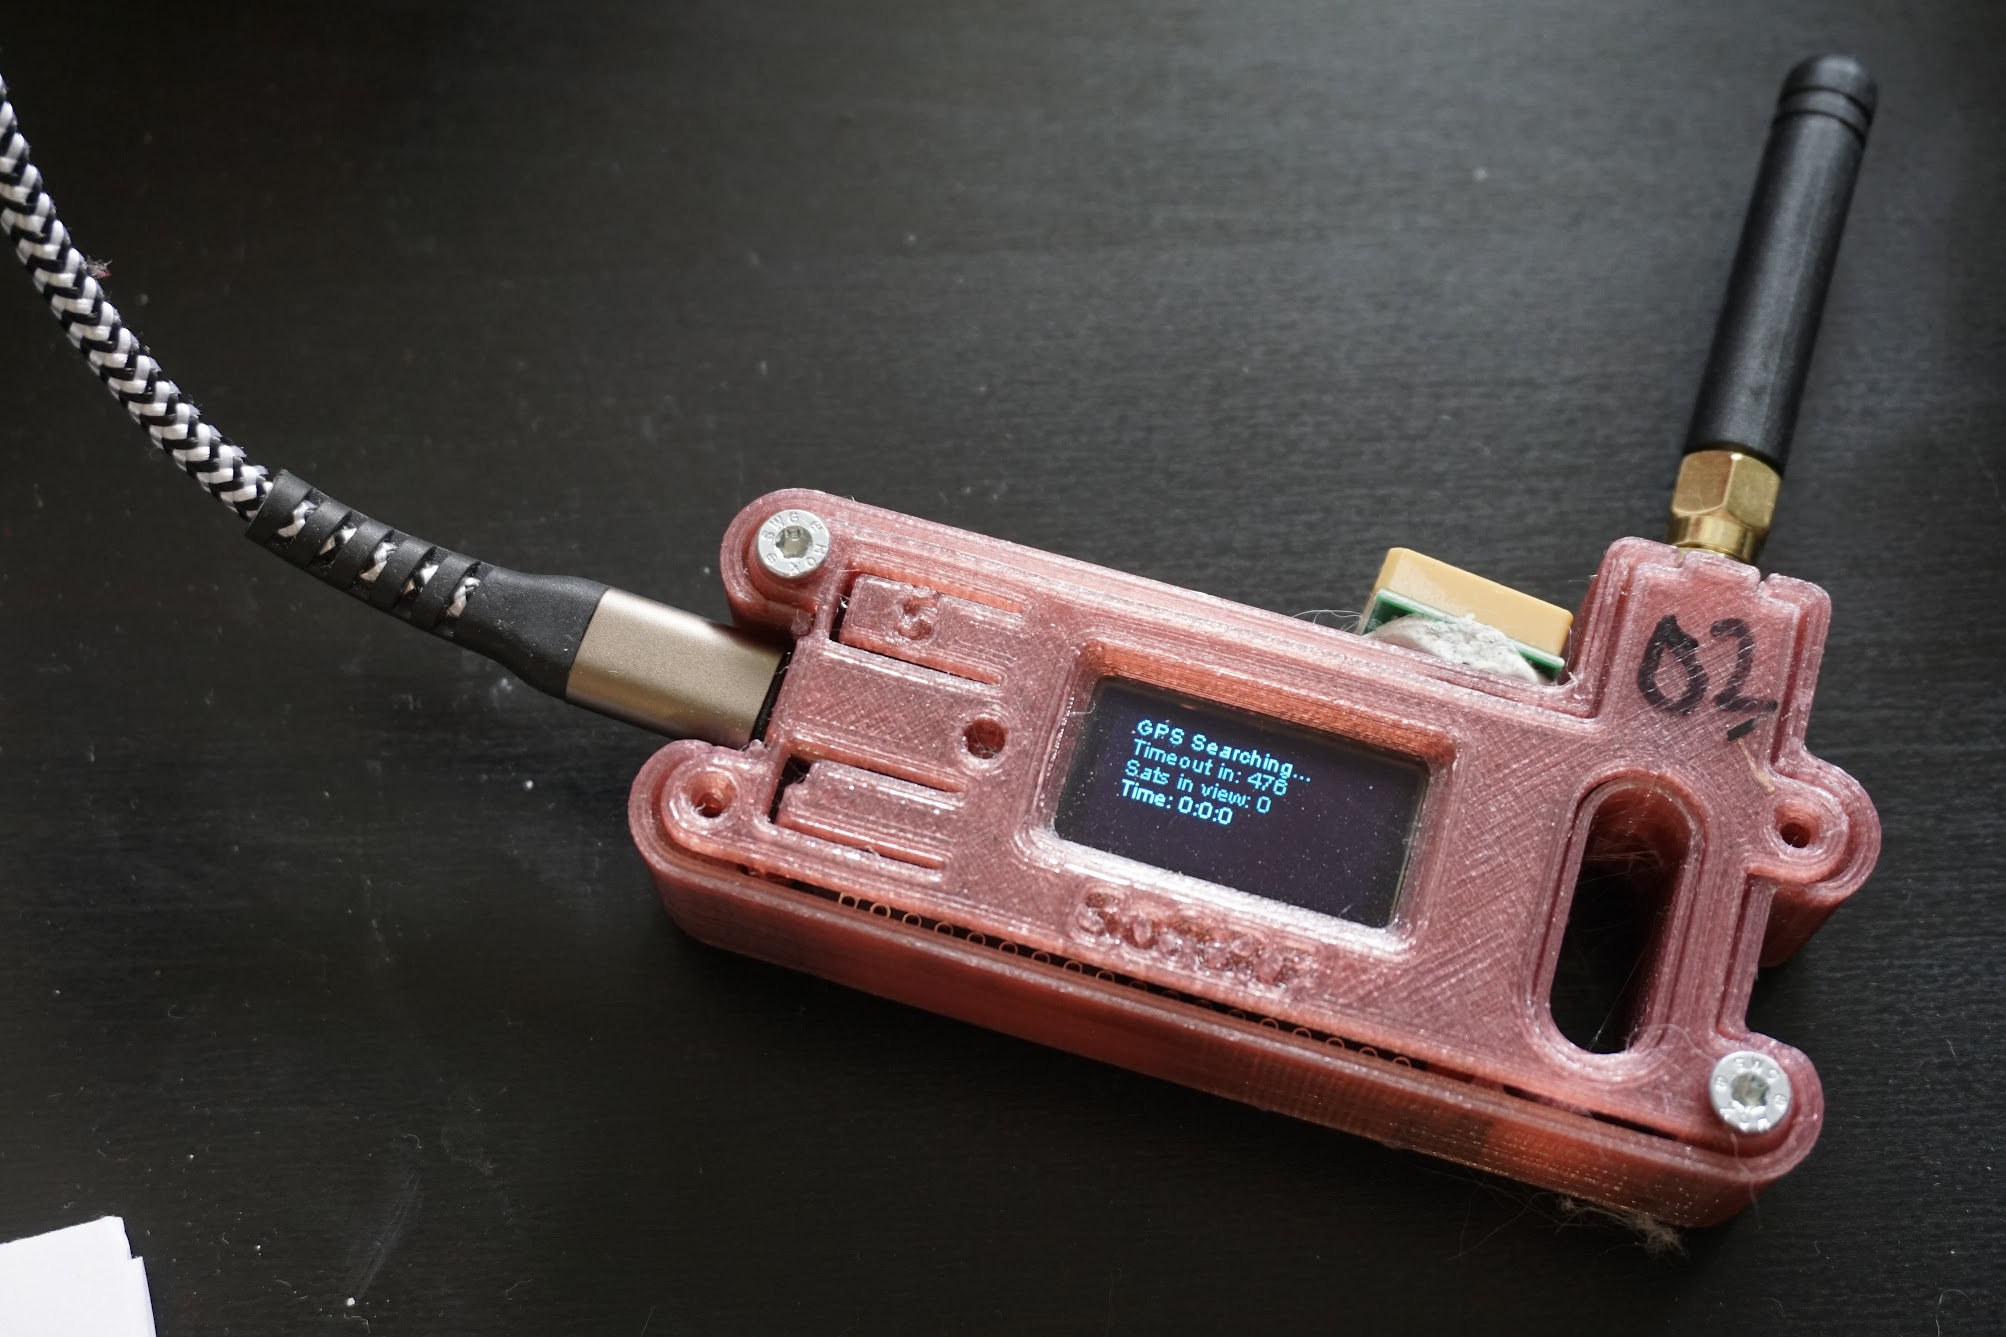
\includegraphics[width=1\textwidth]{pictures/hardware/gps-nodes/HTCC-AB02S.jpg}
        \caption{
            One of the Heltec HTCC-AB02S \ac{LoRaWAN} devices used during this thesis.
            The \acs{OLED} display as well as the \ac{GPS} module as well as the \ac{LoRaWAN} antenna on the top right can be seen.
        }\label{pic:heltec-htcc-ab02s}
    \end{subfigure}%
    ~
    \begin{subfigure}[t]{0.5\textwidth}
        \centering
        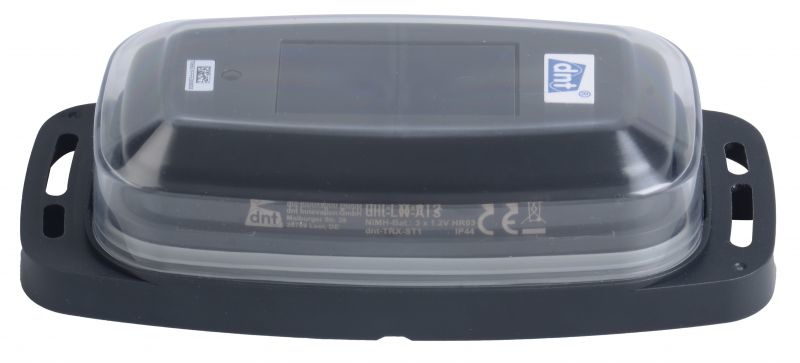
\includegraphics[width=1\textwidth]{pictures/hardware/gps-nodes/dnt-LW-ATS.jpg}
        \caption{
            The dnt-LW-ATS \ac{LoRaWAN} node~\protect\cite{dnt_gmbh_dnt_nodate}.
            The solar module for power harvesting is between the two white labels on the top of the device.
        }\label{pic:dnt-lw-ats}
    \end{subfigure}

    \caption{Pictures of some more end devices.}
\end{figure*}

The combination of the \ac{LoRa} module, the \ac{GPS} module and an \ac{OLED} screen is interesting, though.

\subsubsection{dnt-LW-ATS}

At first glance, this was the most promising \ac{LoRa} node for the task at hand.
It has a built-in \ac{GPS} module as well as a weatherproof, IP44 rated exterior case and a solar panel for charging the internal battery.

However, the node was challenging to set up and operate.
The device offers a \emph{motion based cyclic} mode in which, during physical movement, the node sends its \ac{GPS} coordinates to \ac{TTN} every few seconds.
This, however, did not work in practice and the node would only send its coordinates irregularly, if at all.
The documentation was not helpful with finding the root cause and the manufacturer could only offer to replace the hardware.

\subsubsection{``blinkeding'' --- Arduino with Shield from Prof.\ Zahoransky}

Prof.\ Zahoransky provided an Arduino with a \ac{LoRa} shield that was also used as a \ac{GPS} tracker for this thesis.
Its main advantage is that, being an Arduino, it is easy to program and use.
The frequency of the \ac{GPS} fixes was only several seconds and it could therefore produce a lot of data in a short amount of time.

\subsection{\acl{TTNM} heatmap view before additional data collection}

\begin{figure}[htbp]
    \centering
    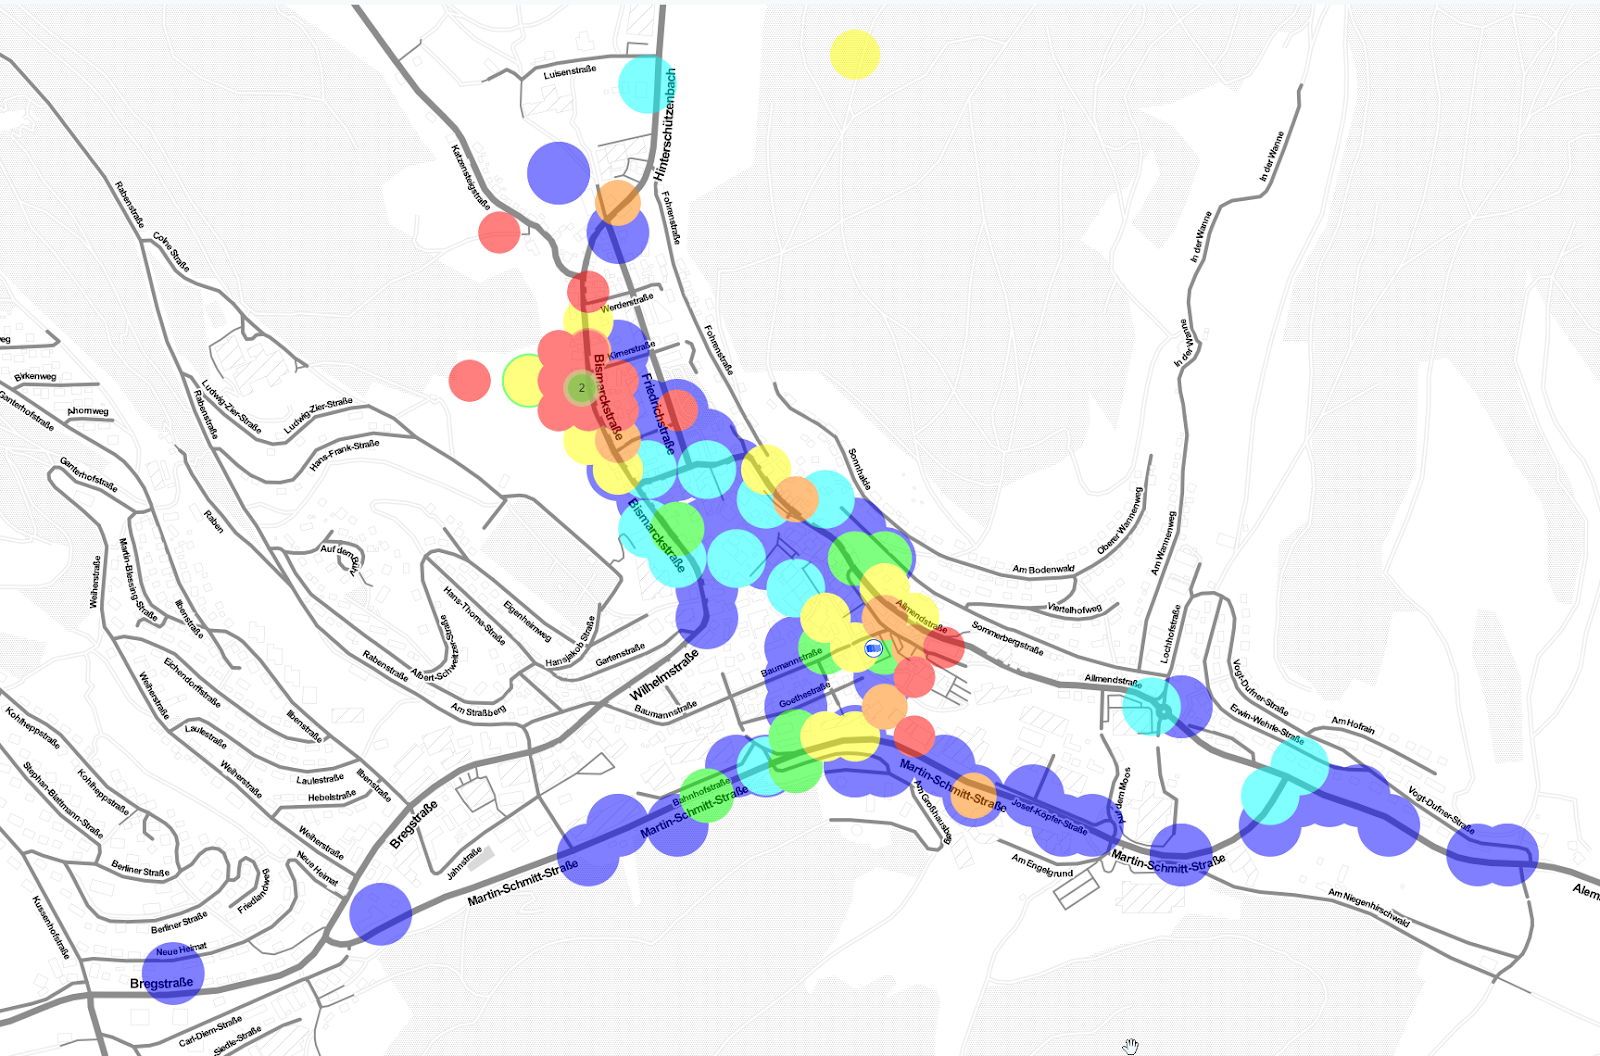
\includegraphics[width=0.8\textwidth]{pictures/ttn-mapper/ttnmapper_heatmap_before.png}
    \caption{
        The \ac{TTNM} heatmap view before additional data collection during this thesis~\cite{ttn_mapper_ttn_2023}.
    }\label{pic:ttnm-before-data-collection}
\end{figure}

\Cref{pic:ttnm-before-data-collection} shows the \ac{TTNM} heatmap view before additional data collection during this thesis.
As mentioned in \cref{sec:collecting-additional-ttnm-data}, additional data needed to be collected in order to be able to create better fingerprinting results.
\Cref{sec:ttm_heatmap_after} shows the heatmap view after additional data collection.

\section{Used development tools}

This section will give an overview over some development tools used for the \ac{TTNL} application.

\subsection{\emph{Docker} and \emph{Docker Compose}}

To simplify deployment and development, \emph{Docker} and \emph{Docker Compose} were used extensively~\cite{docker_inc_docker_2022}\cite{docker_inc_docker_2023}.
Docker allows for applications to be run in lightweight containers that are isolated from the rest of the system.
This allows for easy deployment of applications without having to worry about the underlying system.

In this thesis, Docker was used to containerize the \ac{TTNL} application.
The backend and frontend each have their own \emph{Dockerfiles} that state how these applications should be built.

\begin{figure}[htbp]
    \centering
    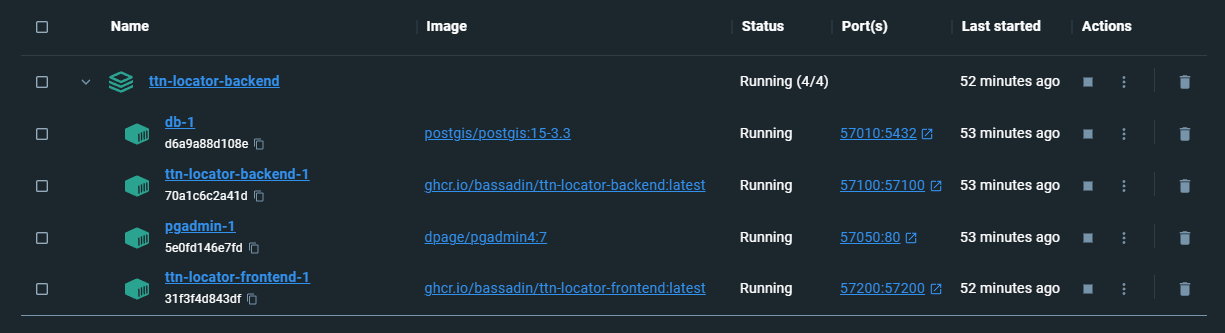
\includegraphics[width=1\textwidth]{pictures/ttn-locator/docker_desktop.png}
    \caption{
        A screenshot of the \emph{Docker Desktop} application that shows the running containers of the \ac{TTNL} application~\cite{docker_inc_download_2021}.
        The \acl{PSQL} \ac{DB} as well as the pgadmin management container are visible as well.
    }\label{pic:docker-desktop}
\end{figure}

Docker Compose was then used to assemble the different parts of the application: the backend, frontend, \acl{PSQL} \ac{DB} and \emph{pgadmin}, an admin interface to make viewing \acl{PSQL} data easier.
\Cref{pic:docker-desktop} shows the running containers of the \ac{TTNL} application in the \emph{Docker Desktop} application~\cite{docker_inc_download_2021}.

\subsection{\acf{VSC}}

\acf{VSC} is a free and open source code editor developed by Microsoft~\cite{microsoft_visual_2023}.
It was chosen as the main code editor for this thesis because of its popularity and the large amount of extensions available for it.

\subsubsection{Extensions}

Of the several extensions that \ac{VSC} offers, some notable ones that helped development during this thesis are listed below.

\paragraph{GitHub Copilot}

GitHub Copilot is an extension that uses \ac{ML} to suggest code snippets based on the current context~\cite{github_inc_github_2023}.
It makes repetitive coding tasks easier and faster by suggesting code snippets that can be inserted with a single keystroke.
It was used extensively during this thesis, both in programming and in the actual writing of this thesis, as it can also autocomplete normal English sentences instead of just code.

\paragraph{PlatformIO}

PlatformIO is a plugin that enables the development of embedded systems with \ac{VSC}~\cite{platformio_platformio_nodate}.
It allows for a user to use \ac{VSC} instead of having to rely on the \emph{Arduino IDE}.

PlatformIO was used in this thesis to develop code for some of the \ac{LoRaWAN} devices used for data collection, for example for the \emph{Heltec HTCC-AB02S} mentioned in \cref{subsubsec:heltec-htcc-ab02s}.

\subsection{GitHub Actions}

\emph{GitHub Actions} is a feature of the \emph{GitHub} platform that allows for automated \ac{CI/CD} workflows to be run on the platform~\cite{github_inc_features_2023}.
These automated workflows can be triggered by various events, such as a new commit being pushed to the repository or a new pull request being opened.

In this thesis, \emph{GitHub Actions} was used to automatically test the \ac{TTNL} frontend and backend as well as build their respective \emph{Docker} images.
These docker images are then pushed to the \emph{GitHub} container registry and can be pulled from there to be deployed.
This allows for the built images to be used in \emph{Docker compose} files on the deployment server without having to build them there.

\section{Program structure: \acf{TTNL}}\label{section:ttnl}

The programmatic implementation of this thesis was called \acf{TTNL} and split into two parts: the backend and the frontend.

\subsection{Overview}

This section aims to give an overview over the program structure of the \ac{TTNL} application.
It also includes the \ac{LoRaWAN} gateways, devices and other parts such as the \ac{TTN} \ac{LNS} in the explanation of the data flow.

\begin{figure}[htbp]
    \centering
    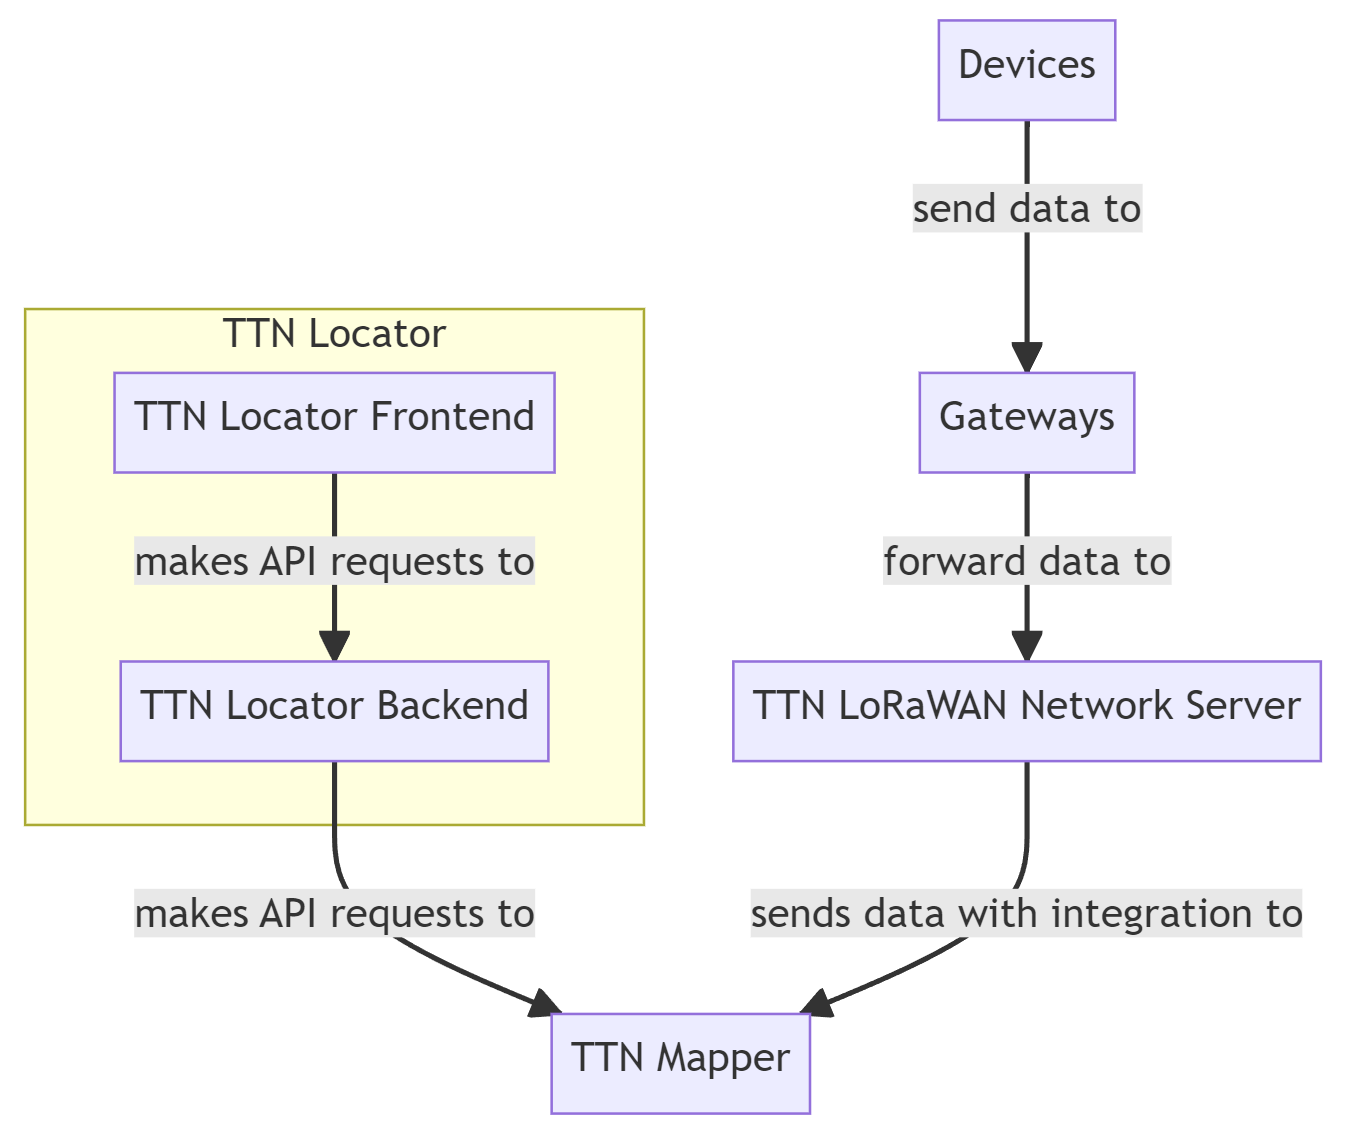
\includegraphics[width=0.7\textwidth]{pictures/ttn-locator/program_structure.png}
    \caption{
        The program structure and data flow of the \ac{TTNL} application as a flowchart.
        \ac{TTNL}, the part that was created during this thesis, is highlighted in yellow.
        The diagram was made with Mermaid~\cite{mermaid_mermaid_2023}.
    }\label{pic:program-structure}
\end{figure}

\Cref{pic:program-structure} shows the program structure and data flow of the \ac{TTNL} application as a flowchart.
The part that was implemented during this thesis is highlighted in yellow.

The data flow starts with the \ac{LoRaWAN} end devices on the right that collect \ac{GPS} data and send it to the \ac{LoRaWAN} gateways using the \ac{LoRaWAN} protocol.
The gateways then forward the packets to the \ac{TTN} \ac{LNS}.
In the Applications section of the \ac{TTN} \ac{LNS}, the \ac{TTNL} application is configured to receive the packets and transform their byte data into a \ac{JSON} format that can be processed by \ac{TTNM}.
Using the \ac{TTNM} integration, \ac{TTN} then sends the data to \ac{TTNM}.

The left side of the diagram shows the \ac{TTNL} application.
The backend periodically fetches the data from \ac{TTNM} via its \ac{REST} \ac{API} and stores it in a \ac{PSQL} \ac{DB}.
The \ac{TTNL} frontend can retrieve data from the backend using a \ac{REST} \ac{API} and present it to the user in various ways.

The following sections will explain each part of the \ac{TTNL} application in detail and show how they were implemented.
The tools and technologies used for the implementation are also explained.

\subsection{Data structure}

\begin{figure}[htbp]
    \centering
    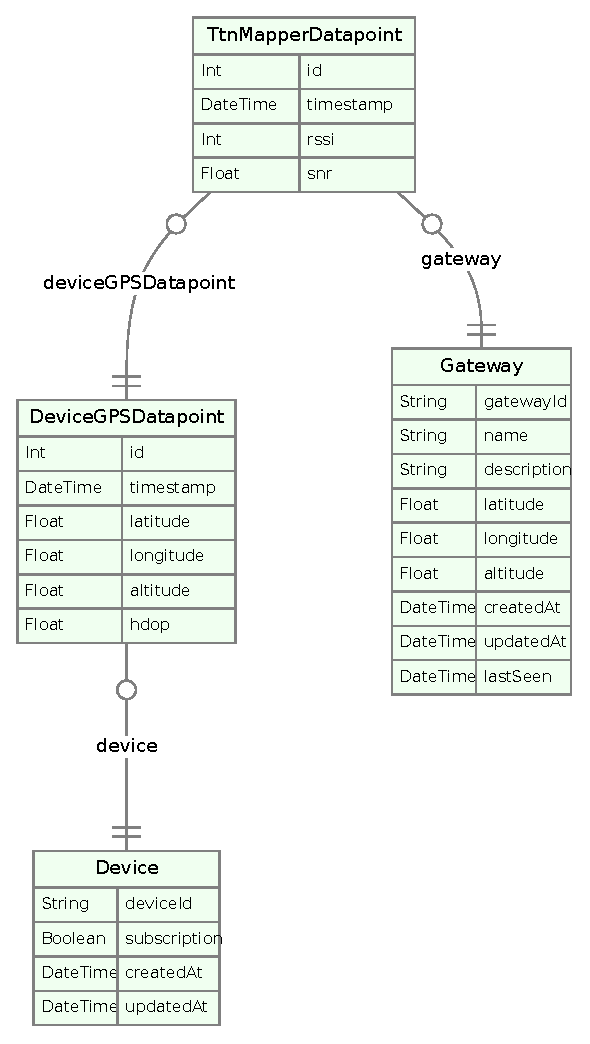
\includegraphics[width=0.4\textwidth]{pictures/ttn-locator/backend/prisma-erd.eps}
    \caption{
        The \ac{DB} structure of the \ac{TTNL} application as an \ac{ERD}.
        The connections between its Device, Gateway, DeviceGPSDatapoint and TtnMapperDatapoint tables are included as well.
        This image was generated using Simon Knott's \emph{Prisma ERD} generator that uses a Prisma schema definition file~\cite{simon_knott_prisma_2023}.
    }\label{pic:prisma-erd}
\end{figure}

\Cref{pic:prisma-erd} shows the \ac{DB} structure of the \ac{TTNL} application as an \ac{ERD}.
It splits up the data received from \ac{TTNM} into four main tables: Device, Gateway, DeviceGPSDatapoint and TtnMapperDatapoint.

\Cref{sec:consolidating-ttnm-data-into-ttnl-db} will describe how the data from \ac{TTNM} was structured to be able to be stored in the \ac{TTNL} \ac{DB} to be able to perform more advanced queries on it.

\subsection{Used technologies --- Backend}

This section describes the technologies used in the backend part of the \ac{TTNL} web application.
The chosen stack uses Express.js with \ac{TS} as the programming language, PostGIS as the \ac{DB} system as well as the Prisma \ac{ORM} to connect to the \ac{DB}.
These services are designed to be running in Docker containers and are orchestrated using Docker Compose.

\subsubsection{\acf{JS} / \acf{TS}}

\ac{JS} is an interpreted, \ac{JIT} compiled programming language that was designed for and is mostly used in web browsers to add interactivity to websites~\cite{mdn_javascript_2023}.
However, it can also be used outside a browser, for example, to create server applications as is explained in \cref{sec:nodejs}.

\ac{TS}, on the other hand, is a superset of \ac{JS} that adds static type checking to the language~\cite{microsoft_javascript_nodate}.
This means that the developer has to specify the types of variables and function parameters, which are then checked by the compiler.
Assigning the wrong type to a variable or passing the wrong type to a function then triggers compile-time error instead of a runtime error.

\begin{lstlisting}[
    language=TypeScript,
    float,
    caption={Example of type checking in \ac{TS}},
    label={lst:example-ts-type-checking}
]
const user = {
    firstName: "Teysa",
    lastName: "Karlov",
    role: "Guildmaster",
}
    
console.log(user.name)
\end{lstlisting}

\Cref{lst:example-ts-type-checking} shows an example of how \ac{TS} can help prevent runtime errors.
The \ac{TS} compiler would show the message \lstinline|Property `name' does not exist on type { firstName: string; lastName: string; role: string; }| since \lstinline{name} is not a property of the \lstinline{user} object.

\subsubsection{Node.js}\label{sec:nodejs}

Node.js is a \ac{JS} runtime environment that allows for the execution of \ac{JS} code outside a web browser~\cite{openjs_foundation_nodejs_nodate}.
It uses the \emph{V8} \ac{JS} engine, which is also used in the Google Chrome web browser~\cite{google_llc_v8_nodate}.
Its main benefit is being able to use a single language for both frontend and backend development --- \ac{JS}, or, in this case, \ac{TS}.

Node.js is available as a Docker image, which makes it easy to use in the Docker Compose setup used in this thesis~\cite{docker_inc_node_2023}.

\subsubsection{Express.js}

Express.js is a ``fast, unopinionated, minimalist web framework for Node.js''~\cite{openjs_foundation_express_nodate}.
``Unopinionated'' means that it does not enforce any specific way of implementing a web application and instead focuses on the premise ``configuration over convention'', leaving the developer to decide how to implement the specifics of the application~\cite{mardan_pro_2014}.

It was used in this thesis as a means to implement the backend part of the \ac{TTNL} web application.
Express.js allows for the creation of \ac{REST} \ac{API} endpoints that can be used by the frontend or by other applications.

\begin{lstlisting}[language=TypeScript, float, caption={Example of an Express.js \ac{API} endpoint}, label={lst:express-api-endpoint}]
router.get('/', async (request: Request, response: Response) => {
    const numberOfDeviceSubscriptions = await GetterFunctions.getAmountOfDeviceSubscriptions();
    response.send({
        message: `Hello from ttn-locator-backend!\nCurrent amount of Device subscriptions: ${numberOfDeviceSubscriptions}`,
    });
});
\end{lstlisting}

\Cref{lst:express-api-endpoint} is an example of an Express.js \ac{API} endpoint that returns a simple message along with the current amount of device subscriptions~\cite{openjs_foundation_express_routing}.
Express also allows for the creation of more complex endpoints that can, for example, return data from a \ac{DB}.
Additionally, routes for different parts of requested data can be defined and put into separate files, making the code more navigable.

\subsubsection{\acf{PSQL} / PostGIS}

\acl{PSQL} (also sometimes simply called \emph{Postgres}) is an open source \ac{RDBMS} that is available for a variety of operating systems~\cite{postgresql_global_development_group_postgresql_2023}.
It is among the most popular \ac{DB} management systems worldwide~\cite{db-engines_most_2023}.

In this thesis, for \ac{TTNL}, \ac{PSQL} was used as the \ac{DB} management system because of its popularity, its possibility to be used with the \ac{ORM} Prisma as well as PostGIS.\
PostGIS is an extension for \ac{PSQL} that adds support for geographic objects and allows for geographic queries~\cite{postgis_psc__osgeo_postgis_2023}.

\begin{lstlisting}[
    language=SQL,
    float,
    caption={
        Example of a PostGIS query to calculate the distance between two geolocation points in meters.
        The result for the two example points would be about 26900.5 meters.
    },
    label={lst:postgis-example-distance}
    ]
SELECT ST_DistanceSphere(
    ST_MakePoint(8.2047, 48.0502), -- Furtwangen
    ST_MakePoint(7.85222, 47.9959) -- Freiburg
);
\end{lstlisting}

\Cref{lst:postgis-example-distance} shows an example of a PostGIS query that calculates the distance in meters between two points on the Earth's surface~\cite{postgis_psc__osgeo_st_distancesphere_nodate}.
It takes into account the curvature of the Earth and is therefore more accurate than using a simple Pythagorean Theorem calculation to determine the distance between two points.

PostGIS is also available as a Docker image, making it easy to deploy in the given docker compose setup~\cite{docker_inc_postgispostgis_2023}.

\subsubsection{Prisma}

Prisma is an \ac{ORM} that can be used with a variety of \ac{DB} management systems, including \ac{PSQL}~\cite{prisma_data_inc_prisma_2023}.
\acp{ORM} allow for the creation of \ac{DB} queries using the programming language of the application instead of using the \ac{DB}'s query language, which would be \ac{SQL} in the case of \ac{PSQL}.\
Instead, Prisma allows for the creation of queries using \ac{TS}.
Prisma also lets the developer define a \ac{DB} schema and can generate migrations to generate the \ac{DB} tables from that schema.

\begin{lstlisting}[
    float,
    caption={
        Example of a Prisma schema.
        It defines two \ac{DB} tables, \lstinline{User} and \lstinline{Post}, as well as their relationship: A User can have many Posts.
    },
    label={lst:prisma-schema-example}
]
model User {
    id    Int     @id @default(autoincrement())
    posts Post[]
}
    
model Post {
    id       Int   @id @default(autoincrement())
    author   User? @relation(fields: [authorId], references: [id])
    authorId Int?
}
\end{lstlisting}

\Cref{lst:prisma-schema-example} shows an example of a Prisma schema that defines two \ac{DB} tables, \lstinline{User} and \lstinline{Post}, and their relationship: A User can have many Posts.

\Cref{pic:prisma-erd} shows a diagram rendered from the Prisma schema that was used in this thesis.

\subsubsection{Vitest}

Vitest is a testing framework for \ac{JS} and \ac{TS}~\cite{vitest_team_vitest-features_2023}.
It was used in this thesis to write unit as well as integration tests for the backend part of the \ac{TTNL} web application.
Vitest uses a syntax that is similar to Chai/Jest, which is a popular syntax for writing tests in \ac{JS} and \ac{TS}~\cite{vitest_team_vitest-features_2023}.

\subsection{Used technologies --- Frontend}

\subsubsection{Vue.js}

Vue.js is a \ac{JS} framework for building reactive user interfaces~\cite{evan_you_vuejs_2023}.
Reactive in this context means the ability for the frontend to automatically react to changes in the \ac{JS}/\ac{TS} state.
It was used in this thesis as a means to implement the frontend of the \ac{TTNL} web application.
Vue can also use \ac{TS} as a programming language, which was used in this thesis for making the code more robust and easier to maintain due to its type safety.

Vue.js was chosen because of the author's previous experience with it and because of its ease of use and quick development time.
It also offers many plugins and libraries that can be used to extend its functionality as well as a large community that can be consulted for help.

\subsubsection{Vuetify}

Vuetify is a \ac{UI} framework for Vue.js that provides Vue components that are based on Google's Material Design guidelines~\cite{vuetify_vuetify_2023}~\cite{google_llc_material_nodate}.
In this thesis, Vuetify was used as a modern looking \ac{UI} framework for the frontend of the \ac{TTNL} web application.
Its usage as import-able predefined Vue components also allowed for a quick and easy implementation of the frontend.

\begin{figure}[htbp]
    \centering
    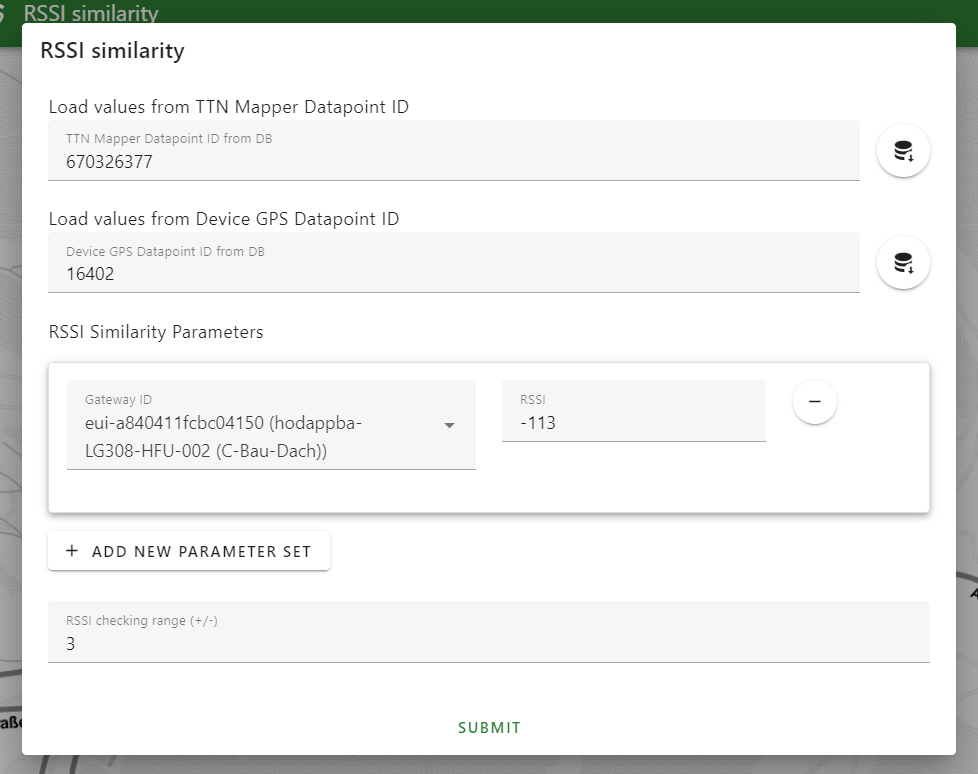
\includegraphics[width=0.8\textwidth]{pictures/ttn-locator/frontend/vuetify-form-example.png}
    \caption{
        An example of a form created using Vuetify components.
        The values of the form fields can be accessed reactively from the Vue component's script part.
    }\label{fig:vuetify-form-example}
\end{figure}

\Cref{fig:vuetify-form-example} shows an example of a form created using Vuetify components in the \ac{TTNL} frontend.
It uses several of Vuetify's components to enable the user to enter \ac{RSS} values for several gateways for localization purposes.

\subsubsection{\acf{OSM}}\label{sec:osm}

\ac{OSM} is a free and open geographic \ac{DB} that relies on a community of volunteers who contribute and update its data through open collaboration~\cite{openstreetmap_contributors_openstreetmap_2023}.
Its use only requires attribution to the \ac{OSM} project and its contributors, which is usually done by placing a small attribution text in a corner of the displayed map.
It was used in this thesis to be able to display a map in the frontend of the \ac{TTNL} application.

\subsubsection{GeoJSON}\label{sec:geojson}

GeoJSON is a format used for representing geographic data using the popular \ac{JSON} format~\cite{butler_geojson_2016}.
This format was used in this thesis as a means to standardize the data format used to represent geographic data as well as its communication between client and server.

\begin{lstlisting}[language=JSON, float, caption={Example of a GeoJSON that represents a rectangle above the furtwangen city center}, label={lst:geojson-example}]
{
    "type": "FeatureCollection",
    "features": [
        {
            "type": "Feature",
            "properties": {},
            "geometry": {
                "coordinates": [
                    [
                        [8.2032444080252, 48.05293370858834],
                        [8.2032444080252, 48.04823334925436],
                        [8.20949460707348, 48.04823334925436],
                        [8.20949460707348, 48.05293370858834],
                        [8.2032444080252, 48.05293370858834]
                    ]
                ],
                "type": "Polygon"
            }
        }
    ]
}  
\end{lstlisting}

\Cref{lst:geojson-example} shows an example of a GeoJSON object.

\subsubsection{Leaflet}\label{sec:leaflet}

Leaflet is a \ac{JS} library for displaying interactive maps in the browser~\cite{volodymyr_agafonkin_leaflet_2023}.
It currently has around 800,000 weekly downloads on the npm package repository~\cite{npm_leaflet_2023}.
It was used in this thesis to display the map on the frontend of the \ac{TTNL} web application.
Leaflets widespread use and large community made it a good choice for this purpose since there are many examples and tutorials available online.

To make Leaflet work with Vue.js, the \emph{vue2-leaflet} plugin was used~\cite{vue_leaflet_team_vue_nodate}.
It wraps Leaflet's functionality into Vue components and provides reactive bindings for Leaflet's properties and map data.

In most cases, an \ac{OSM} map was used to display the data.

Leaflet is able to render GeoJSON objects, as seen in \cref{sec:geojson}.
This was used in this thesis to display some data on the map of the \ac{TTNL} frontend, e.g.,\ the multilateration annuli.

\subsection{Consolidating \acl{TTNM} data into the \acl{TTNL} \acl{DB}}\label{sec:consolidating-ttnm-data-into-ttnl-db}

To be able to perform more advanced queries on the data, it needed to be, partly, transferred into the \ac{TTNL} \acl{DB}.
Since, for the scope of this thesis, only devices that captured data near the Furtwangen area were of interest, only data from those devices was transferred.
This is because fingerprinting on a larger or even global scale would likely result in the need for a much bigger, maybe even distributed \ac{RDBMS}.
However, the \ac{TTNL} application theoretically also allows for any other data to be transferred into the \ac{DB}, as long as that device has been captured by \ac{TTNM} at some point in time.

To collect data from \ac{TTNM}, an \ac{API} endpoint was used that returns all data for a given device in a given time frame.
For example, to get data for a \ac{LoRaWAN} device with the id \emph{blinkeding} from the first week of April 2023, the following \ac{URL} could be used for a GET \ac{HTTP} request: \url{https://api.ttnmapper.org/device/data?dev_id=blinkeding&start_time=2023-04-01T00:00:00.000Z&end_time=2023-04-08T00:00:00.000Z}.
This \ac{TTNM} \ac{API} route returns data in a \ac{JSON} format.
This \ac{JSON} data was parsed and Prisma was used to insert it into the \ac{PSQL} \ac{DB}.

To avoid having to do this importing of data regularly, the \ac{TTNL} backend includes a cronjob task that automatically imports data from \ac{TTNM} every 24 hours.
Cron allows for tasks to be executed at specific times or intervals.
It uses a specific syntax to define these intervals, for example \emph{* */4 * * *} would execute a task every 4 hours~\cite{drake_how_2020}.

The cronjob for importing new data only does this for devices that have been entered into its \ac{DB} by a user to avoid flooding the \ac{DB} with irrelevant data.
This ensures that the \ac{TTNL} \ac{DB} is always up-to-date with the device specific data from the \ac{TTNM} \ac{DB}.

\subsection{Cleaning collected data}\label{subsec:cleaning-collected-data}

The data that was collected by \ac{TTNM} was not without errors and outliers.
\ac{TTNM} filters out some of the data that is sent to it.
For example, it does not accept data points that have a \ac{HDOP} value greater than a certain unspecified amount.
As far as the data collected by \ac{TTNL} is concerned, no \ac{HDOP} values above 5 were recorded, so it is likely that this is the cutoff point.
There were several problems that were noticed when trying to use the data for localization purposes:

\begin{itemize}
    \item \textbf{Outliers:} Some data points were clearly outliers, i.e.,\ the device moved from one location to another one that was far away in a short amount of time.
    \item \textbf{Duplicates:} Some devices were prone to producing/sending duplicate data points.
\end{itemize}

To counteract these problems, another cronjob in the \ac{TTNL} backend was created.
This cronjob runs every few hours and executes a \ac{SQL} query with Prisma's \lstinline|$executeRaw| that removes outliers and duplicates from the \ac{TTNL} \ac{DB}.

\begin{lstlisting}[
    language=SQL,
    float,
    caption={
        Part of the \ac{SQL} query that was used to remove outliers and duplicated from the collected \ac{TTNM} data.
        This section handles the calculation of the speed the end device moved at between the current and the previous datapoint.
        The query was generated by \emph{Bing AI} and adjusted so that it could be used more easily with the existing Prisma \ac{DB} schema.
    },
    label={lst:sql-remove-outliers}
]
CASE
    WHEN prev_latitude IS NOT NULL
    AND prev_longitude IS NOT NULL
    AND prev_timestamp IS NOT NULL THEN ST_DistanceSphere(
        ST_MakePoint(longitude, latitude),
        ST_MakePoint(prev_longitude, prev_latitude)
    ) / EXTRACT(
        EPOCH
        FROM
            (timestamp - prev_timestamp)
    )
    ELSE NULL
END AS speed
\end{lstlisting}

\Cref{lst:sql-remove-outliers} shows the \ac{SQL} code that was used to determine the speed between subsequent data points of the same device.
The PostGIS function \lstinline|ST_DistanceSphere| is used to calculate the distance between the current and the previous data point.

\begin{lstlisting}[
    language=SQL,
    float,
    caption={
        Example of a \ac{SQL} snippet that gets the latitude of the previous \ac{GPS} data point of the same device.
    },
    label={lst:get-preceding-datapoint-sql}
]
LAG(latitude) OVER (PARTITION BY "deviceId" ORDER BY timestamp AS prev_latitude
\end{lstlisting}

In order to get the previous datapoint, the SQL \lstinline|LAG| function was used.
For example, \cref{lst:get-preceding-datapoint-sql} shows a \ac{SQL} snippet that gets the latitude of the previous \ac{GPS} data point of the same device.

Duplicates were removed using a similar approach.
Instead of calculating the distance between the two data points, their latitude, longitude, \ac{HDOP} and altitude values were compared.

\section{Locating \acs{LoRaWAN} devices with multiple techniques}

This section will describe the different techniques used to locate \ac{LoRaWAN} devices in this thesis.

\subsection{\acs{RSSI}-based multilateration}\label{sec:rssi-based-multilateration-implementation}

The general idea behind using \ac{RSS} values to determine the distance to a gateway is simple.
The \ac{RSSI} value measured by a gateway is inversely proportional to the distance between the device and the gateway.
The further away a device is from a gateway, the lower (or more negative) the \ac{RSSI} value will be.
This correlation was explained in \cref{sec:background-free-space-path-loss}.

\begin{figure}[htbp]
    \centering
    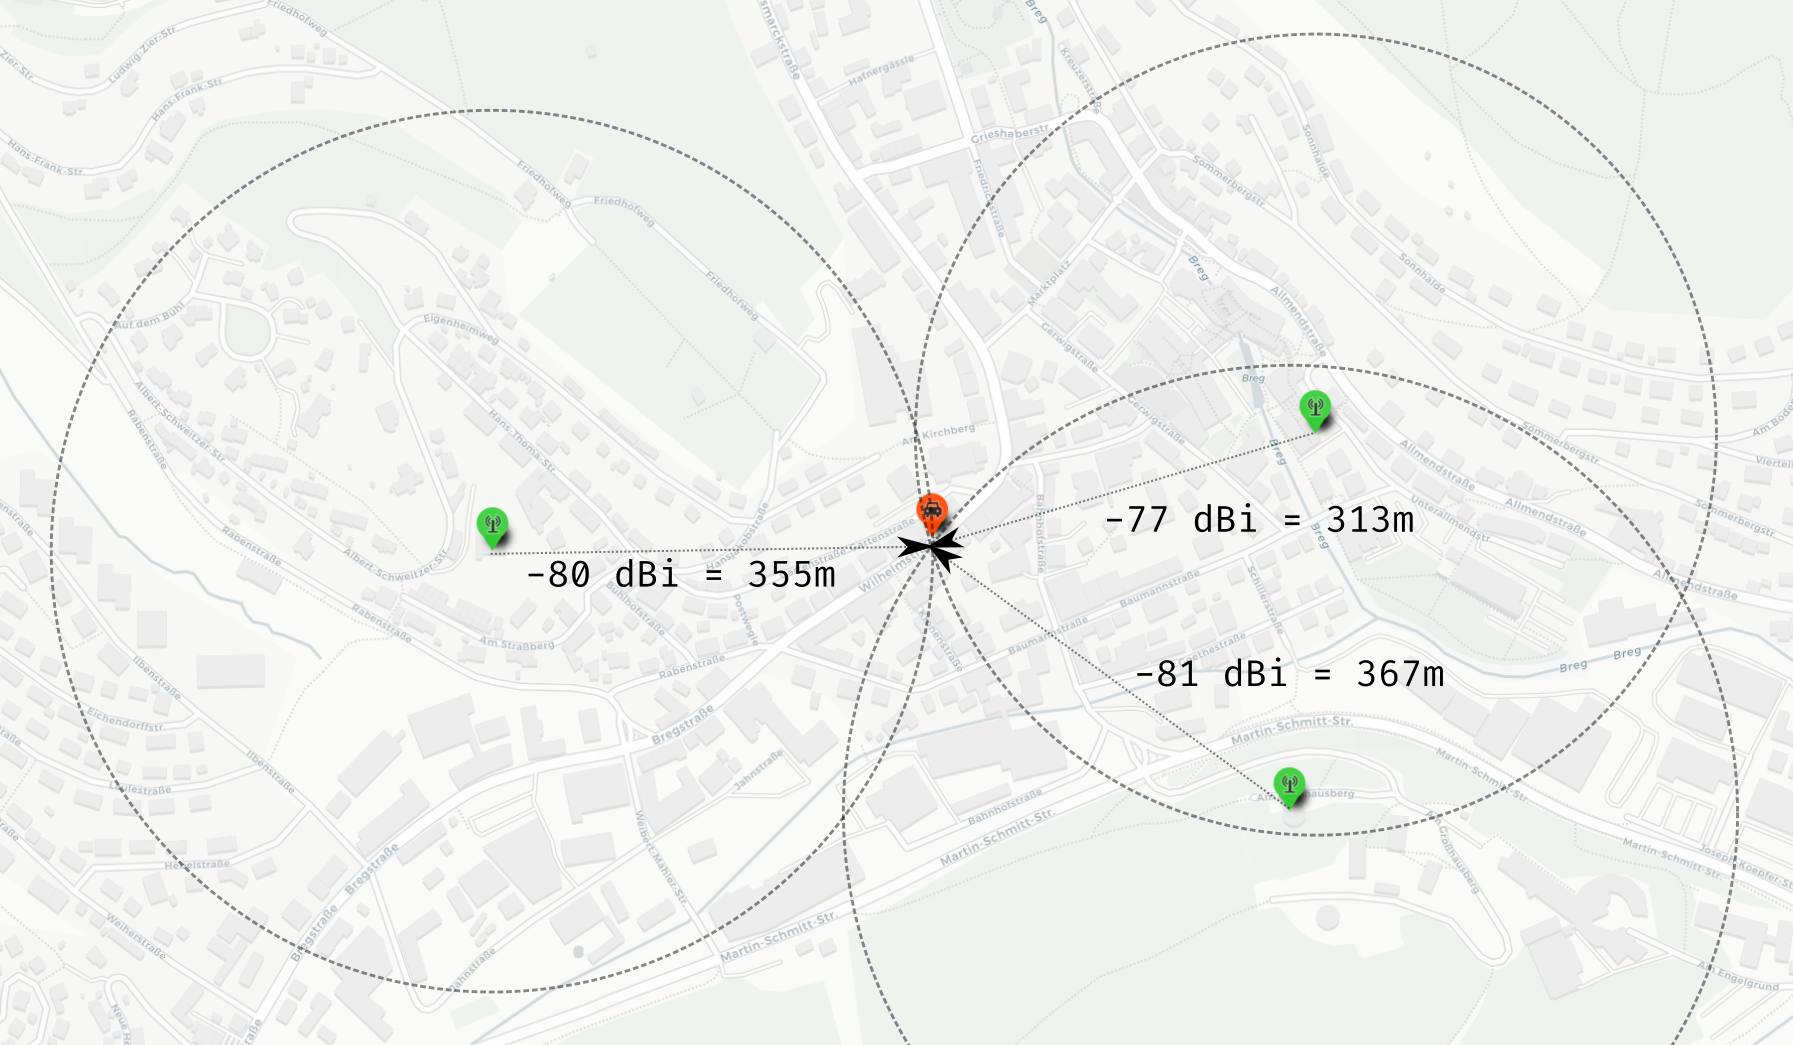
\includegraphics[width=1\textwidth]{pictures/multilateration/rssi-multilateration-example.png}
    \caption{
        An example of the theory behind mapping \ac{RSS} values to distances using three gateways, based on the correlation explained in \cref{sec:background-free-space-path-loss}.
        The device (orange pin) is located at the intersection of the three circles originating from the gateways (green pins).
        \ac{RSS} values that are received by the gateways are inversely proportional to the distance between the device and the gateway.
        They are used to calculate the distance between the device and the gateway, making a multilateration possible.
        The map was generated using the \ac{OSM} based tool \emph{umap}~\cite{noauthor_umap_nodate}.
    }\label{fig:rssi-multilateration-theoretical-example}
\end{figure}

\Cref{fig:rssi-multilateration-theoretical-example} shows an example of how \ac{RSS} values can be used to determine the location of a device.
A fact to take note of is that the \ac{RSSI} values measured by \ac{TTN} are only integers and not floating point numbers.
This lowers the accuracy of the calculated distances and therefore the accuracy of the calculated location of the device.

Based on these facts, several attempts were made to calculate the distance between a device and a gateway.

\subsubsection{First idea: Fixed \acs{RSSI} to range scale}\label{sec:fixed-rssi-to-range-scale}\label{sec:fixed-rssi-to-range-scale-impl}

The first idea for determining the distance between a device and a gateway was to use a fixed \ac{RSSI} to range scale.
This means that for a given \ac{RSSI} value, a range is determined by inputting said \ac{RSSI} value into a function.
The equation depicted in \cref{eq:fixed-rssi-to-range-scale} shows an example where a \ac{RSSI} value is inputted.
The result is the distance $D_{gateway}$ to the gateway in meters.

\begin{equation}\label{eq:fixed-rssi-to-range-scale}
    D_{gateway} = -12 * rssi - 605
\end{equation}

For example, a \ac{RSSI} value of -80 would result in a distance of \SI{355}{\meter}.
A value of -110 would result in a distance of \SI{715}{\meter}.

The values for this equation were derived by performing a linear regression on the \ac{RSS} values of the device-based GPS data points from the MikroTik LR8 gateway deployed on top of the \ac{GHB} 2 building.
While those values work well for the \ac{RF} reception behavior of the gateway that was used to derive them, they are not necessarily applicable to other gateways.
Hence, one single fixed \ac{RSSI} to range scale function is not suitable to be used for all gateways as their position (indoor/outdoor) as well as their antennas might be different from one another.

Although rare, \ac{RSS} values that are larger than a certain threshold can also return negative range values.
In the example above, this is the case with values $>= -50$.

Another problem, as mentioned in \cref{sec:rssi-based-multilateration}, is that the \ac{MPP} phenomenon can cause the \ac{RSS} values to fluctuate, even when end device, gateway, and the distance between them stay the same.
This makes RSSI values in general a rather unreliable metric for determining the distance between a device and a gateway as long as there is no \ac{LoS} between them.

\subsubsection{Plotting \acs{RSSI} to range from existing data}\label{sec:plotting-rssi-to-range-from-existing-data}

\Cref{fig:rssi-range-graph-positive-example} shows an example of a \ac{RSSI} to distance graph that the frontend of \ac{TTNL} generated.
It uses the \ac{RSS} values of the device-based data points from a single gateway to generate the graph by calculating the distance to said gateway.
This makes it possible to determine the values of a linear regression function that can be used to calculate the distance to a gateway from a given \ac{RSSI} value.
Compared to the fixed \ac{RSSI} to range scale described in \cref{sec:fixed-rssi-to-range-scale}, this approach has the advantage that it can be used to generate a more accurate \ac{RSSI} to range scale by considering each gateway's behavior individually.
The example in \cref{fig:rssi-range-graph-positive-example} works quite well for this.

\begin{figure}[htbp]
    \centering
    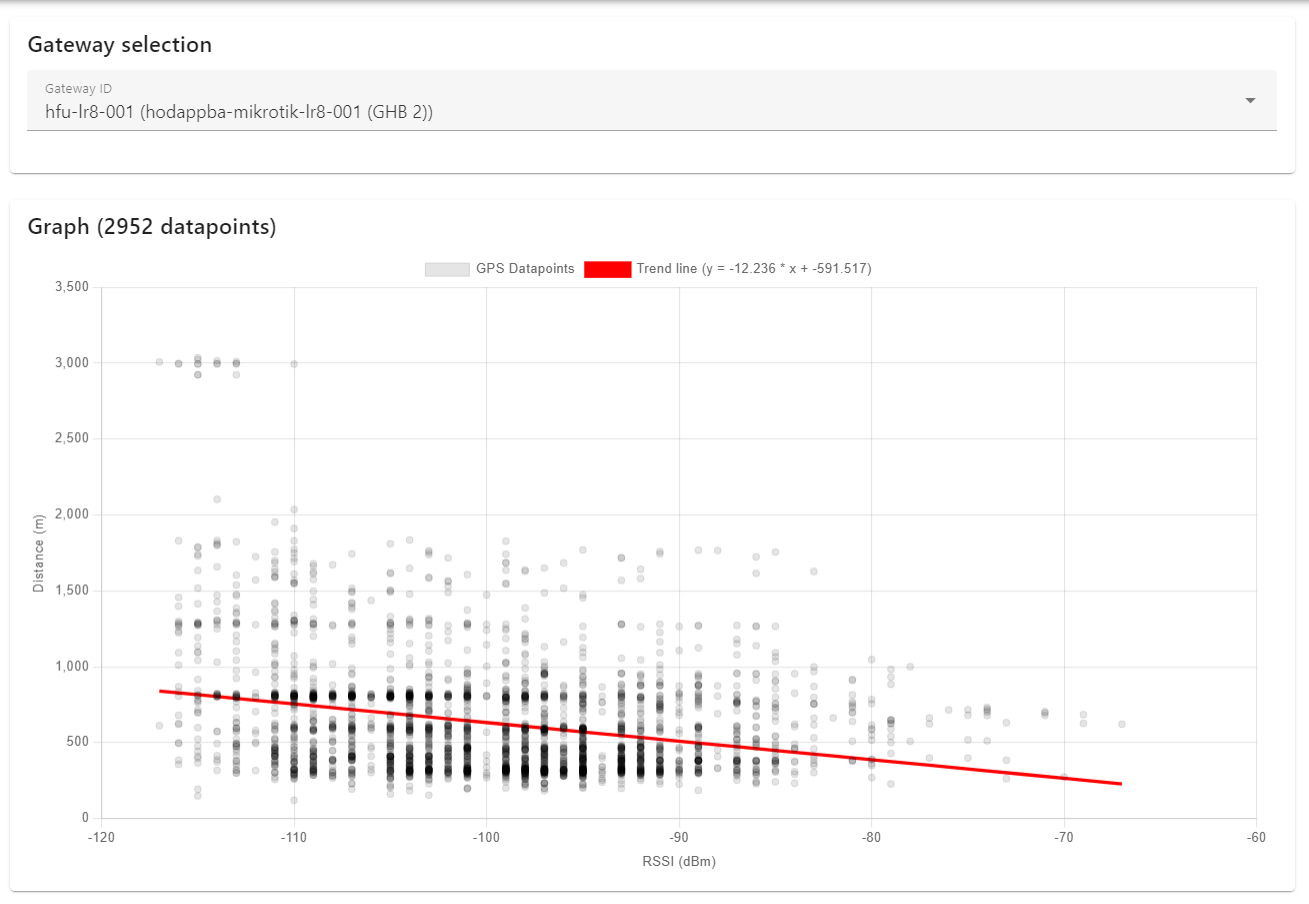
\includegraphics[width=0.8\textwidth]{pictures/ttn-locator/frontend/data/gateway_ghb_rssi_range_graph.png}
    \caption{
        Screenshot from the \ac{TTNL} frontend showing a positive example of a \ac{RSSI} to distance graph.
        Some outliers are visible in the upper left of the graph.
    }\label{fig:rssi-range-graph-positive-example}
\end{figure}

While there are outliers in the data, the graph still shows a logical average linear correlation between the \ac{RSS} values and their distance where the \ac{RSS} values decrease as the distance increases.

\begin{figure}[htbp]
    \centering
    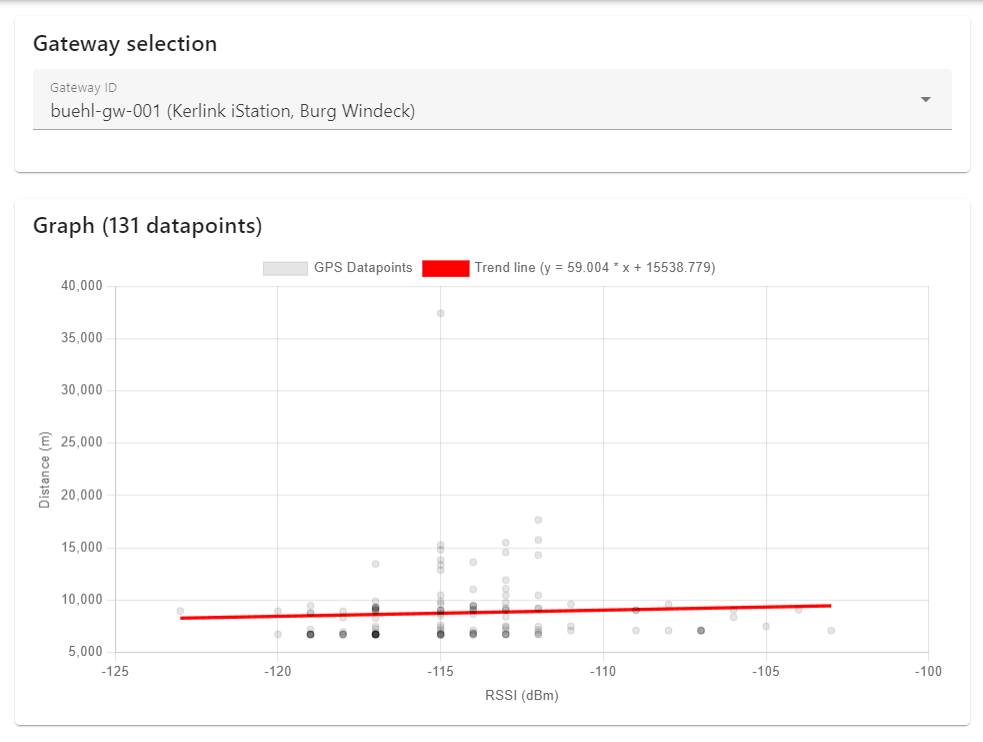
\includegraphics[width=0.8\textwidth]{pictures/ttn-locator/frontend/data/gateway_buehl_gw_rssi_range_graph.png}
    \caption{
        Screenshot from the \ac{TTNL} frontend showing a negative example of a \ac{RSSI} to distance graph.
        The \ac{RSS} values do not decrease as the distance increases in this case.
        It is possible that this is caused by not enough data points being available as compared to the positive example in \cref{fig:rssi-range-graph-positive-example}.
    }\label{fig:rssi-range-graph-negative-example}
\end{figure}

\Cref{fig:rssi-range-graph-negative-example} shows another example of a \ac{RSSI} to distance graph that the frontend of \ac{TTNL} generated.
In this example, the \ac{RSS} values do not decrease as the distance increases.
This could have several reasons, such as not enough data points being available (the negative example has only 131 vs.\ almost 3,000 for the positive example).

\Cref{subsubsec:conclusion-rssi-linear-regression} will discuss the results of using this technique and the resulting accuracy in more detail.

\subsubsection{Using existing data to build a per-gateway \acs{RSSI} to range scale}\label{subsubsec:per-gateway-rssi-to-range-scale}

Using a similar linear regression approach as described in \cref{sec:plotting-rssi-to-range-from-existing-data}, a per-gateway \ac{RSSI} to range scale was realized.
As was mentioned in that chapter, this allows for gateway-specific parameters such as positioning and antenna type to be taken into account.

The Gateway table in the \ac{DB} was extended two include two more columns: \texttt{linear\-Regres\-sion\-Slope} and \texttt{linear\-Re\-gres\-sion\-Inter\-cept} for the slope and the y axis intercept of the linear regression function, respectively.
This was only done for gateways with more than 500 ttnMapperDatapoints in the \ac{DB} to avoid outliers skewing the results like in \cref{fig:rssi-range-graph-negative-example}.
While the approach in \cref{sec:plotting-rssi-to-range-from-existing-data} calculated the regression client-side, this approach calculates the regression server-side and stores the results in the \ac{DB} for more efficient access.
\Cref{lst:sql-calculate-linear-regression} shows the \ac{SQL} query that was used to calculate those linear regression values.
Again, a cron-like job was used since recalculating those linear regression values for all gateways each time a new data point was received would be too resource intensive.

\begin{lstlisting}[
    language=SQL,
    float,
    caption={
        \ac{SQL} query that was used to calculate the linear regression values for each gateway.
        Using the \texttt{UPDATE} and \texttt{SET} statements, the results of the subquery are written into the \texttt{linear\-Re\-gres\-sion\-Slope} and \texttt{linear\-Re\-gres\-sion\-Inter\-cept} columns of the Gateway table for the corresponding gateways.
        This caption was once more generated by Bing AI and adapted for better readability.
    },
    label={lst:sql-calculate-linear-regression}
]
UPDATE "Gateway"
SET "linearRegressionSlope" = subquery.slope,
    "linearRegressionIntercept" = subquery.intercept
FROM (
    SELECT
        "Gateway"."gatewayId",
        regr_slope(
            ST_DistanceSphere(
                ST_MakePoint("Gateway"."longitude", "Gateway"."latitude"),
                ST_MakePoint("DeviceGPSDatapoint"."longitude", "DeviceGPSDatapoint"."latitude")),
            "TtnMapperDatapoint"."rssi"
        ) AS slope,
        regr_intercept(
            ST_DistanceSphere(
                ST_MakePoint("Gateway"."longitude", "Gateway"."latitude"),
                ST_MakePoint("DeviceGPSDatapoint"."longitude", "DeviceGPSDatapoint"."latitude")),
            "TtnMapperDatapoint"."rssi"
        ) AS intercept
    FROM "Gateway"
    JOIN "TtnMapperDatapoint" ON "TtnMapperDatapoint"."gatewayId" = "Gateway"."gatewayId"
    JOIN "DeviceGPSDatapoint" ON "DeviceGPSDatapoint"."id" = "TtnMapperDatapoint"."deviceGPSDatapointId"
    GROUP BY "Gateway"."gatewayId"
    HAVING COUNT(*) >= 500
) AS subquery
WHERE "Gateway"."gatewayId" = subquery."gatewayId";
\end{lstlisting}

When requesting gateway data from the backend, it answers with the linear regression values for each gateway.
The frontend then uses these values to display annuli around each gateway on the map according to specific \ac{RSSI} values.
If a gateway does not have linear regression values set in the \ac{DB} (possibly due to not having enough ttnMapperDatapoints yet), the frontend will fall back to the fixed \ac{RSSI} to range scale described in \cref{sec:fixed-rssi-to-range-scale}.

\Cref{subsubsec:conclusion-rssi-linear-regression} will show the results of using this technique and the accuracy improvements in more detail.

\subsubsection{Plotting \acs{SNR} to range from existing data}\label{sec:plotting-snr-to-range-from-existing-data}

Similar to \cref{sec:plotting-rssi-to-range-from-existing-data}, an attempt was also made to plot \ac{SNR} values to range from existing data, instead of the \ac{RSS}.

\begin{figure}[htbp]
    \centering
    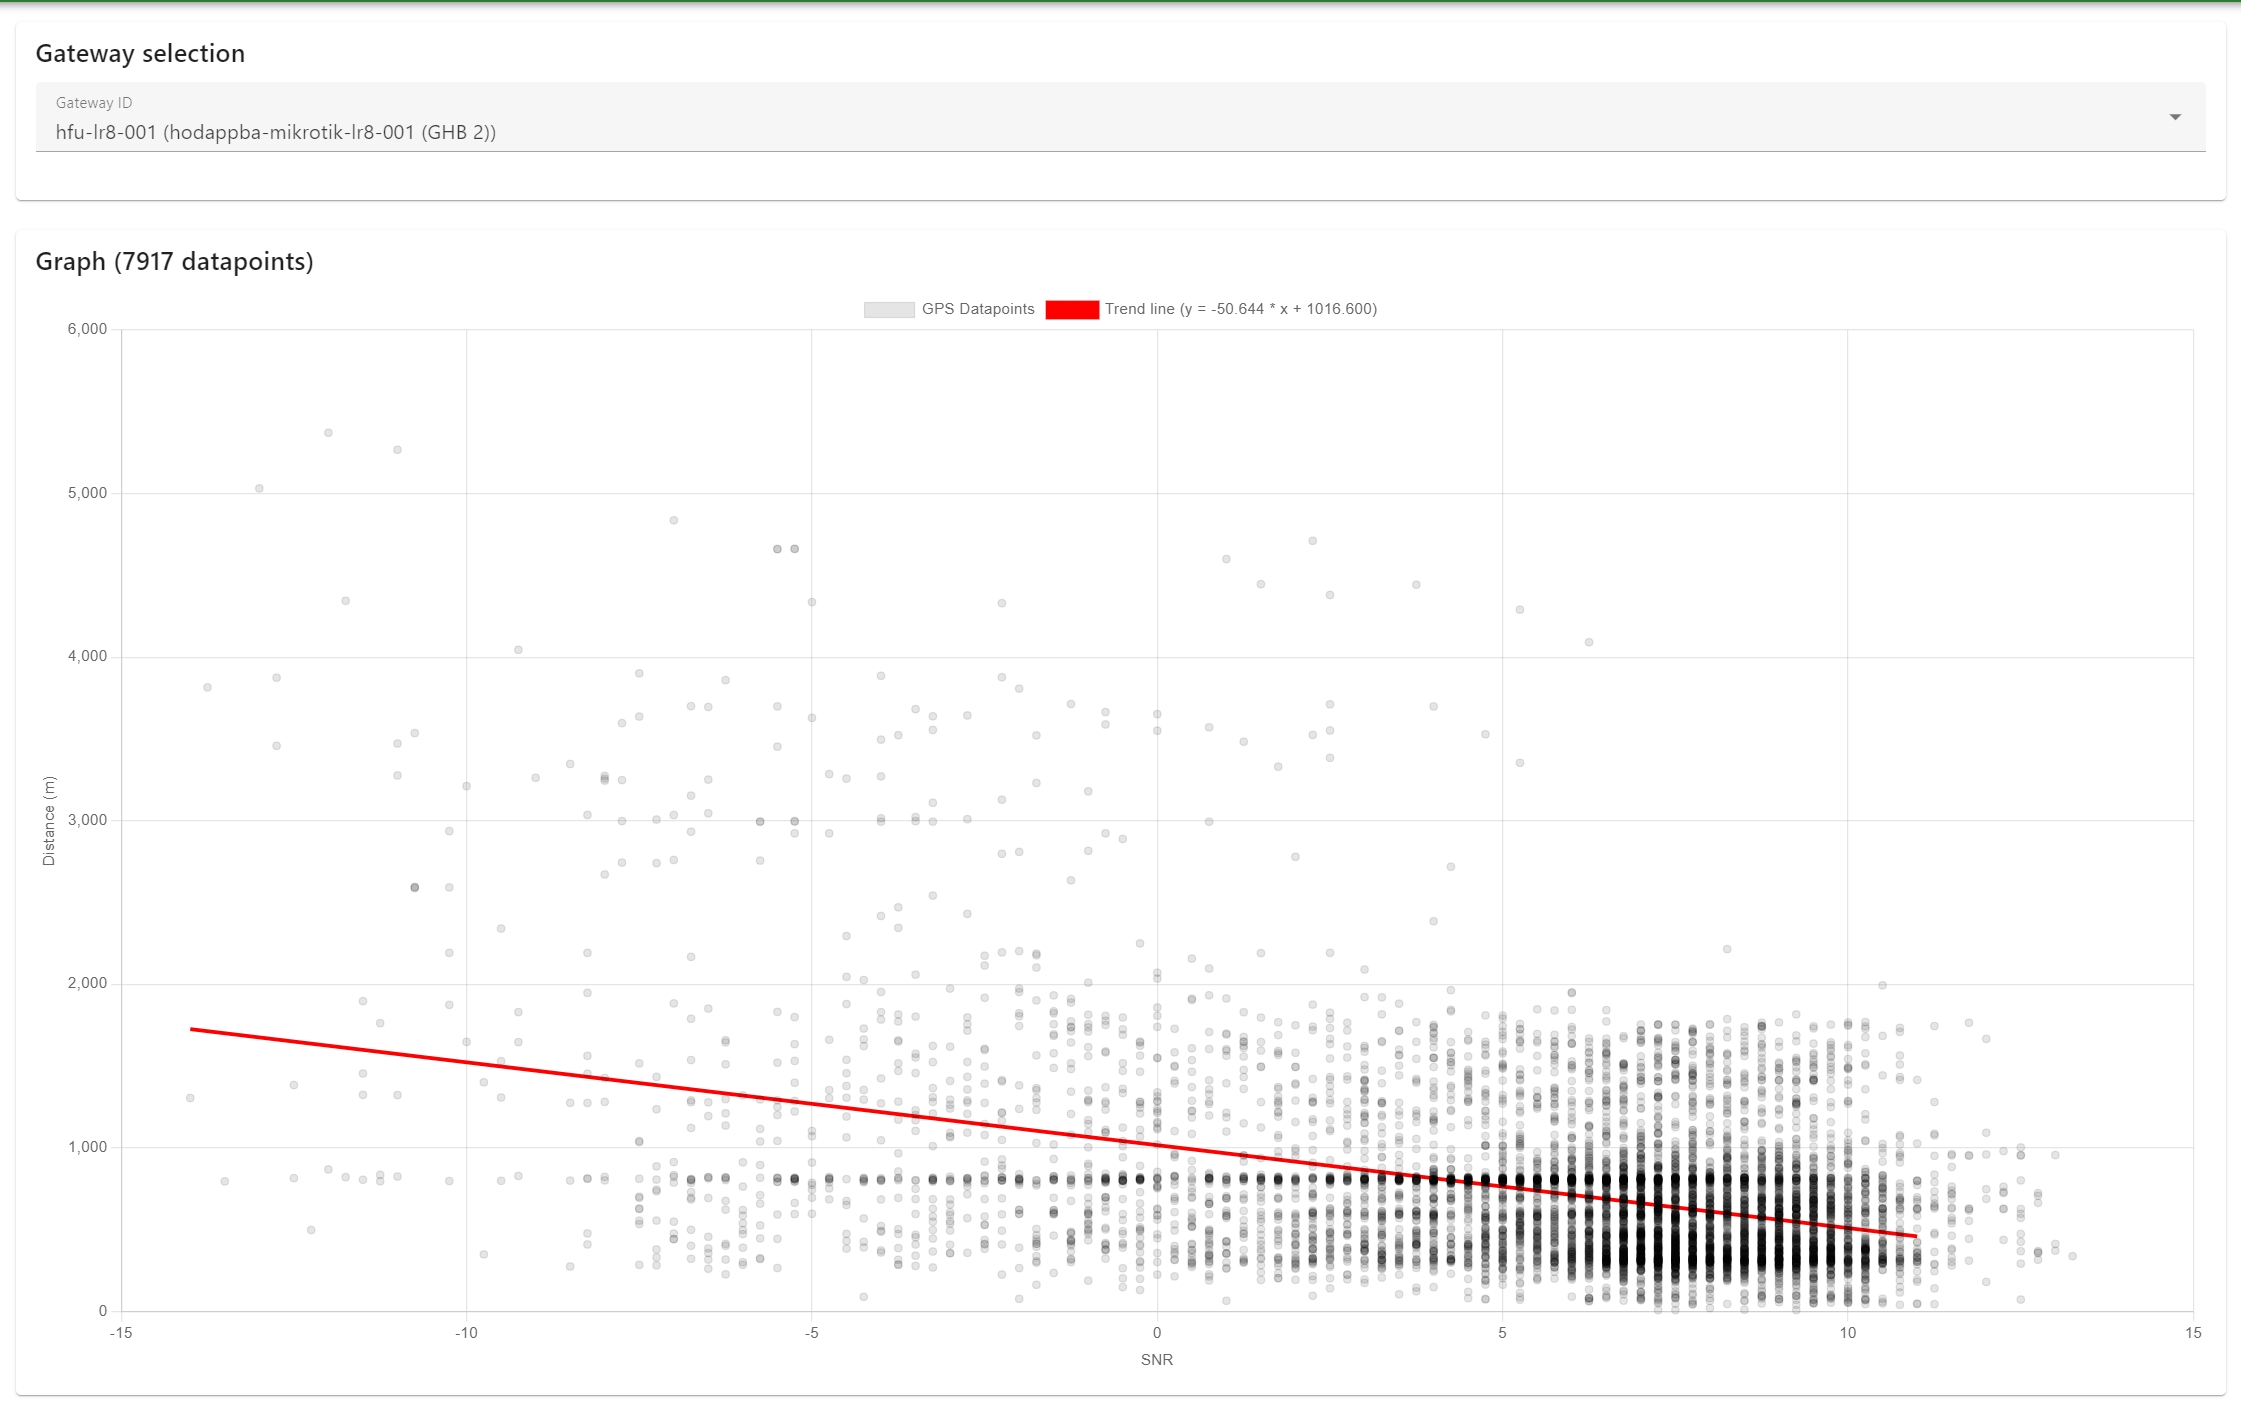
\includegraphics[width=0.8\textwidth]{pictures/ttn-locator/frontend/data/gateway_ghb_snr_range_graph.jpg}
    \caption{
        Screenshot from the \ac{TTNL} frontend showing an example of a \acf{SNR} to distance graph.
        While the graph shows an attempt at fitting a linear regression function to the data, it is not accurate, since there is no strong linear correlation between \ac{SNR} and distance either.
        Many outliers can be seen, making this approach unreliable as well.
    }\label{fig:snr-range-graph-example}
\end{figure}

\Cref{fig:snr-range-graph-example} shows an example of this, using data from the \ac{GHB} gateway.
Compared to \cref{fig:rssi-range-graph-positive-example}, the graph also shows a rather weak correlation between \ac{SNR} and distance similar to that between \ac{RSSI} and distance.

However, mapping \ac{SNR} values to distance on their own seemed very unreliable.
This is to be expected, since, as was explained in \cref{sec:background-snr}, the \ac{SNR} value can be influences by many things, such as external factors and the environment even more so than the \ac{RSS} value.

To plot the graphs, data points with varying \acp{SF} were used.
Since a higher \ac{SF} also allows for signals with worse \ac{SNR} to be received, as explained in \cref{sec:sf-snr-correlation}, this could have also influenced the results.

\subsection{\acf{ToA}-based multilateration}\label{subsec:toa-based-multilateration-implementation}

One of the seemingly most promising techniques for locating \ac{LoRaWAN} devices is \ac{ToA}-based multilateration.
As has been explained in \cref{sec:toa-based-multilateration}, this technique uses the time of arrival of a \ac{LoRa} signal to multiple gateways to calculate the position of the device that sent the signal using the speed of light.

Unfortunately, this technique did not work as expected in the scope of this thesis.
This was because the timestamps of signal arrival in the gateways that were used for this thesis were not accurate enough.
Differences of up to 1 second between the timestamps of the same signal in different gateways were not uncommon, making distance calculations using these values utterly unusable.

\begin{figure}[htbp]
    \centering
    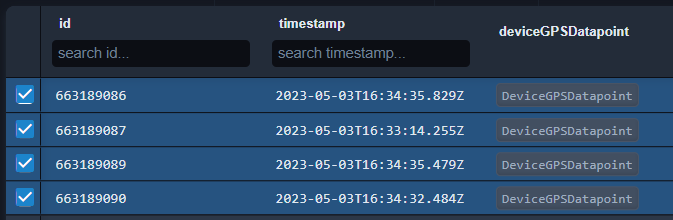
\includegraphics[width=0.7\textwidth]{pictures/multilateration/toa_bad_data_example_prisma_studio.png}
    \caption{
        Picture taken from Prisma's \emph{Prisma Studio} web frontend.
        Example of divergent timestamp data that was planned to be used for \ac{ToA} multilateration.
        The time difference between the first and second signal arrival amounts to more than one second.
    }\label{fig:toa-bad-data-example}
\end{figure}

\Cref{fig:toa-bad-data-example} shows an example of the divergent timestamp data that was planned to be used for \ac{ToA} multilateration where the time difference between the first and second signal arrival amounts to more than one second.
Since the speed of light is $299792458\ \mathrm{m/s}$, a difference of one second in the timestamps of two signals would result in a distance difference of $299792458\ \mathrm{m}$.
This is a distance that is way too big to be useful for performing any sort of meaningful multilateration.

\Cref{subsec:conclusion-toa-tdoa} will explain how this could be fixed.

\subsection{Fingerprinting with \acs{RSSI} and other values}\label{sec:fingerprinting-implementation}

The implementation of the fingerprinting approach was done in the backend part of \ac{TTNL}.
A \ac{REST} endpoint was added to the backend that accepts a list of gateway IDs along with maximum and minimum \ac{RSS} values for those particular gateways.

\begin{lstlisting}[
    language=TypeScript,
    float,
    caption={
        Part of the Prisma query that filters the fingerprint data points by their similarity to the \ac{RSS} values of gateways provided by the frontend.
    },
    label={lst:prisma-rssi-fingerprinting-query}
]
const prismaFilterQuery: any = {
    AND: [],
};

for (const filterCriteria of similarityFilter) {
    prismaFilterQuery.AND.push({
        ttnMapperDatapoints: {
            some: {
                gateway: {
                    gatewayId: filterCriteria.gatewayId,
                },
                rssi: {
                    gte: filterCriteria.minRssi,
                    lte: filterCriteria.maxRssi,
                },
            },
        },
    });
}

return prisma.deviceGPSDatapoint.findMany({ where: prismaFilterQuery });
\end{lstlisting}

\Cref{lst:prisma-rssi-fingerprinting-query} shows part of that code from the \ac{TTNL} backend.
By iterating over the \lstinline|similarityFilter| array provided by the frontend, the backend can add a \lstinline|AND| clause to the Prisma query for each gateway data entry that was provided by the frontend.
These \lstinline|AND| clauses are then put into a Prisma \lstinline|findMany| query with a where clause that is executed against the \ac{DB}.
The query returns all deviceGPSDatapoints that have ttnMapperDatapoints that match the gateway ID and \ac{RSSI} range provided by the frontend.

\begin{figure}[htbp]
    \centering
    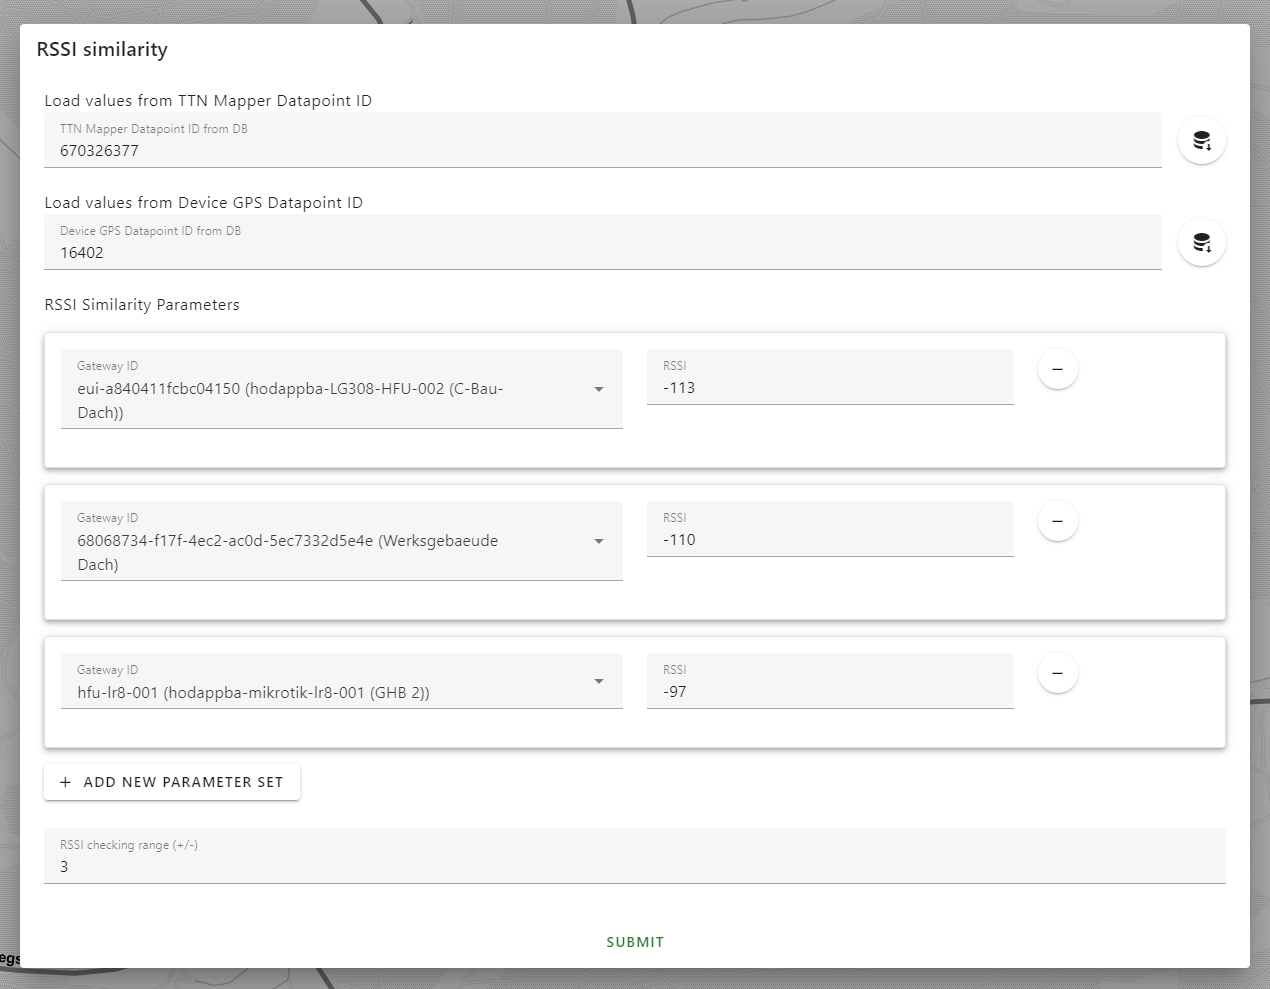
\includegraphics[width=0.7\textwidth]{pictures/ttn-locator/frontend/rssi_similarity_form.png}
    \caption{
        Screenshot of the \ac{TTNL} frontend showing the form for entering gateway fingerprinting values.
        The top of the form shows the possibility of entering \ac{TTNM} datapoint IDs to load their respective similarity values from the \ac{DB}.
        A ``RSSI'' checking range of 3 has been set, meaning that the entered \ac{RSS} values will be checked against the \ac{RSS} values of the \ac{TTNM} datapoints with a tolerance of 3.
        For example, since the first gateway selected has an \ac{RSSI} value of -113, all \ac{TTNM} datapoints with an \ac{RSSI} value between -116 and -110 of that gateway will be matched.
    }\label{fig:rssi-similarity-form-frontend}
\end{figure}

\Cref{fig:rssi-similarity-form-frontend} shows the frontend form for entering gateway fingerprinting values to be sent to the backend.

\begin{figure}[htbp]
    \centering
    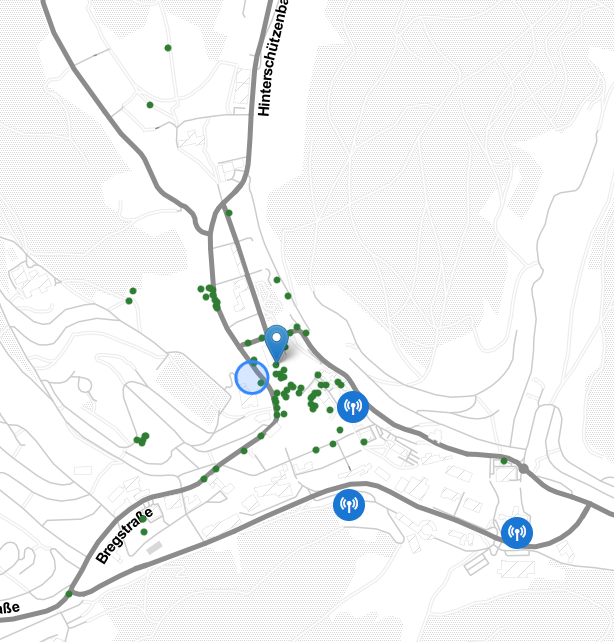
\includegraphics[width=0.6\textwidth]{pictures/ttn-locator/frontend/fingerprinting/rssi_similarity_map_example.png}
    \caption{
        Screenshot of the \ac{TTNL} frontend showingan example for a fingerprinting result map generated by \ac{TTNL}.
        The blue pin shows the actual position of the device.
        The blue circle (arbitrary radius) shows the position that \ac{TTNL} calculated out of the center of the matching datapoints.
    }\label{fig:fingerprinting-map-example-only-center}
\end{figure}

\ac{TTNL} can show the matching datapoints on its map as can be seen in \cref{fig:fingerprinting-map-example-only-center}.
The blue pin shows the actual position of the device.
To calculate a position estimate, \ac{TTNL} takes the center of the matching datapoints and draws a circle around it with an arbitrary radius.

This was improved later by fitting the radius of the estimated position circle to half of the matching datapoints.
An explanation will be given in \cref{subsubsec:conclusion-rssi-linear-regression}.

\subsubsection{Adding \acf{SNR} and \acf{SF} to fingerprinting}\label{sec:adding-snr-to-fingerprinting}

In an attempt to make fingerprinting results more accurate, the \ac{SNR} value of the \ac{TTNM} datapoints was added to the fingerprinting algorithm in addition to the raw \ac{RSSI} values.
Since \ac{TTN} captures \ac{SNR} and \ac{SF} with each forwarded package anyway, this didn't affect the diffficulty of data collectionand only required adding an extra column to the \ac{DB} schema.

\cref{subsec:conclusion-fingerprinting} will show the improvements that each of those approaches brought.